\documentclass[a4paper, oneside]{book}
\usepackage{graphicx} % Required for inserting images
\usepackage{emptypage}
\usepackage{array}
\usepackage{hyperref}
\usepackage{listings}
\usepackage{xcolor}
\usepackage{makecell}

\lstdefinestyle{javaStyle}{
    language=Java,
    basicstyle=\ttfamily\small,
    keywordstyle=\color{blue}\bfseries,
    stringstyle=\color{green!50!black},
    commentstyle=\color{gray},
    morecomment=[l][\color{magenta}]{\#},
    numbers=left,
    numberstyle=\tiny\color{gray},
    frame=single,
    breaklines=true,
    breakatwhitespace=false,
    showstringspaces=false
}
\lstset{
    style=javaStyle,
    breaklines=true,
    breakatwhitespace=false,
    linewidth=0.95\textwidth  % Slightly narrower than text width
}

\usepackage{tabularray}
\usepackage{tabularx}
\usepackage{adjustbox}

\usepackage{float}

\renewcommand{\chaptername}{}
\renewcommand{\contentsname}{Indice}

\author{R. Regina, F. Rossetti, F. Trotti}
\title{DietiEstates25}
\date{April 2025}

\begin{document}

\maketitle

\tableofcontents

\chapter{Versioni}
\begin{center}
\begin{tabular}{| m{8em} | m{8cm}|}
    \hline
    Versione & Modifiche \\
    \hline
    1.0 & Prima versione. \\
    \hline
\end{tabular}
\end{center}

\subsection{Panoramica del documento}
DietiEstates25 é un software che:
\begin{list}{$\cdot$}{}
    \item permette alle agenzie immobiliari di gestire in modo facile
    ma completo ed efficace il proprio business.
    \item allow real estates agencies to manage in a easy yet 
    complete and powerful way their business.
    \item allow people to effectively find and buy/rent a 
    real estate.
\end{list}

\subsection{Glossario}
\begin{center}
\begin{tabular}{| m{8em} | m{8cm}|}
    \hline
    Manager & Un componente di amministrazione dell'agenzia immobiliare 
    che si occupa di gestire gli agenti dell'agenzia. \\
    \hline
    Administrator & L'unico manager con privilegi. E' gerarchicamente 
    elevato rispetto agli altri manager.
    \\
    \hline
    Agent & Un agente immobiliare appartenente ad un'agenzia immobiliare 
    che si occupa di gestione degli annunci e delle relazioni con i clienti (customers). \\
    \hline
    Property & Un bene immobile, ovvero un bene stabilmente fisso che non è 
    possibile spostare, che può essere sia un fabbricato che un terreno.\\
    \hline
    Lising & Un annuncio pubblicato da un agente che descrive la messa in 
    vendita/affitto di un immobile. \\
    \hline
    Customer & Una persona che desidera acquistare/affittare un immobile.\\
    \hline
    Tour & Visita dell'immobile concordata tra cliente ed agente al fine del 
    suo eventuale acquisto/affitto.\\
    \hline
    Personal data & I dati che un utente ha inserito in fase di registrazione: 
    e-mail, telefono, nome, cognome \dots \\
    \hline

\end{tabular}
\end{center}

\subsection{System Environment}
% \includegraphics{} % use case diagram


\chapter{Specifica dei requisiti}
\section{Requisiti funzionali}
In questa sezione si vanno a specificare, secondo il rigoroso 
formalismo tabellare di A. Cockburn due degli use case ritenuti 
più significativi e centrali.
\subsection{Ricerca Immobili}
% Per tabelle che occupano più di una pagina:
%  longtblr al posto di tblr
\begin{longtblr}[
    caption = {Diagramma di Cockburn del caso d'uso \textit{Ricerca Immobili}.}
]{
    width = 10cm, %per fissare una larghezza
    column{1} = {3cm},
    column{2} = {0.8cm},
    column{3-4} = {3cm},
	vlines = {}, %per le cornici verticali
	hlines = {}, %per le cornici orizzontali
    % Merge delle righe/colonne:
    cell{1-7}{2} = {c = 3}{10cm, halign = l},
    cell{8}{1} = {r = 7}{valign = t},
    cell{15}{1} = {r = 3}{valign = t},
    cell{18}{1} = {r = 5}{valign = t},
    cell{23}{1} = {r = 2}{valign = t},
    cell{25}{1} = {r = 3}{valign = t},
    cell{28}{1} = {r = 3}{valign = t},
    cell{31}{1} = {r = 3}{valign = t},
    cell{34}{2} = {c = 3}{10cm, halign = l}
}
USE CASE & Ricerca Immobili & & \\
Goal in Context & Il Cliente vuole trovare annunci di immobili di suo interesse. & & \\
Preconditions & Nessuna precondizione. & & \\
Success End Condition & Il sistema tiene traccia della ricerca effettuata, salvandola tra le “Ricerche recenti”. & & \\
Fail End Condition & Il sistema tiene traccia della ricerca effettuata, salvandola tra le “Ricerche recenti”. & & \\
Primary Actor & Cliente & & \\
Trigger & Il Cliente clicca sulla barra di ricerca della schermata principale. & & \\
Main Scenario & Step & Cliente & Sistema   \\
 & 1 & Trigger & \\
 & 2 & & Mostra: 
 le eventuali ricerche recenti;
 la ricerca tramite punto sulla mappa. \\
 & 3 & Inserisce testo nella barra di ricerca.
 Seleziona il tipo di annuncio.
 Clicca su “Cerca”. & \\
 & 4 & & Mostra la schermata completa di ricerca. Mostrando i risultati. \\
 & 5 & Clicca su un risultato. & \\
 & 6 & & Mostra in sovrimpressione la schermata dettagliata dell’annuncio. Termina use case. \\
Extension A: 
click su una ricerca recente & Step & Cliente & Sistema \\
 & 3.a & Clicca su una ricerca recente. & \\
 & 4.a & & Torna allo step 4 del main scenario. \\
Extension B: 
ricerca tramite punto sulla mappa. & Step & Cliente & Sistema \\
 & 3.b & Clicca su “Ricerca tramite punto sulla mappa”. & \\
 & 4.b & & Mostra la schermata di ricerca tramite punto sulla mappa. \\
 & 5.b & Seleziona un punto sulla mappa, specificando un raggio di ricerca e clicca conferma. & \\
 & 6.b & & Torna allo step 4 del main scenario. \\

\pagebreak
Extension C:
la ricerca non ha prodotto risultati. & Step & Cliente & Sistema \\
 & 4.c & & Mostra la schermata “Non sono stati trovati risultati”. Torna allo step 2 del main scenario. \\
Extension D: nessun testo inserito.
 & Step & Cliente & Sistema \\
 & 3.d & non inserisce testo nella barra di ricerca e clicca su “Cerca”. & \\
 & 4.d & & Mostra messaggio “Inserisci una zona o un indirizzo”. Torna allo step 2 del main scenario. \\
Extension E: applica filtri. & Step & Cliente & Sistema \\
 & 5.e & Modifica dei filtri di ricerca. & \\
 & 6.e & & Torna allo step 4 del main scenario. \\
Extension F: annulla ultima operazione & Step & Cliente & Sistema \\
 & 5.b.f & Clicca sul pulsante annulla & \\
 & 6.b.f & & Torna allo step 2 del main scenario. \\
Open Issues & \begin{list}{+}{}
    \item Modellare o meno la barra di ricerca superiore?
    \item Modellare o meno il ritorno alla home con il click sul logo? E’ possibile scrivere una cosa del tipo Step:tutti per intendere che può avvenire in ogni step del Cliente?
\end{list} & & \\
\end{longtblr}
\begin{figure}[h]
    \centering
    \fbox{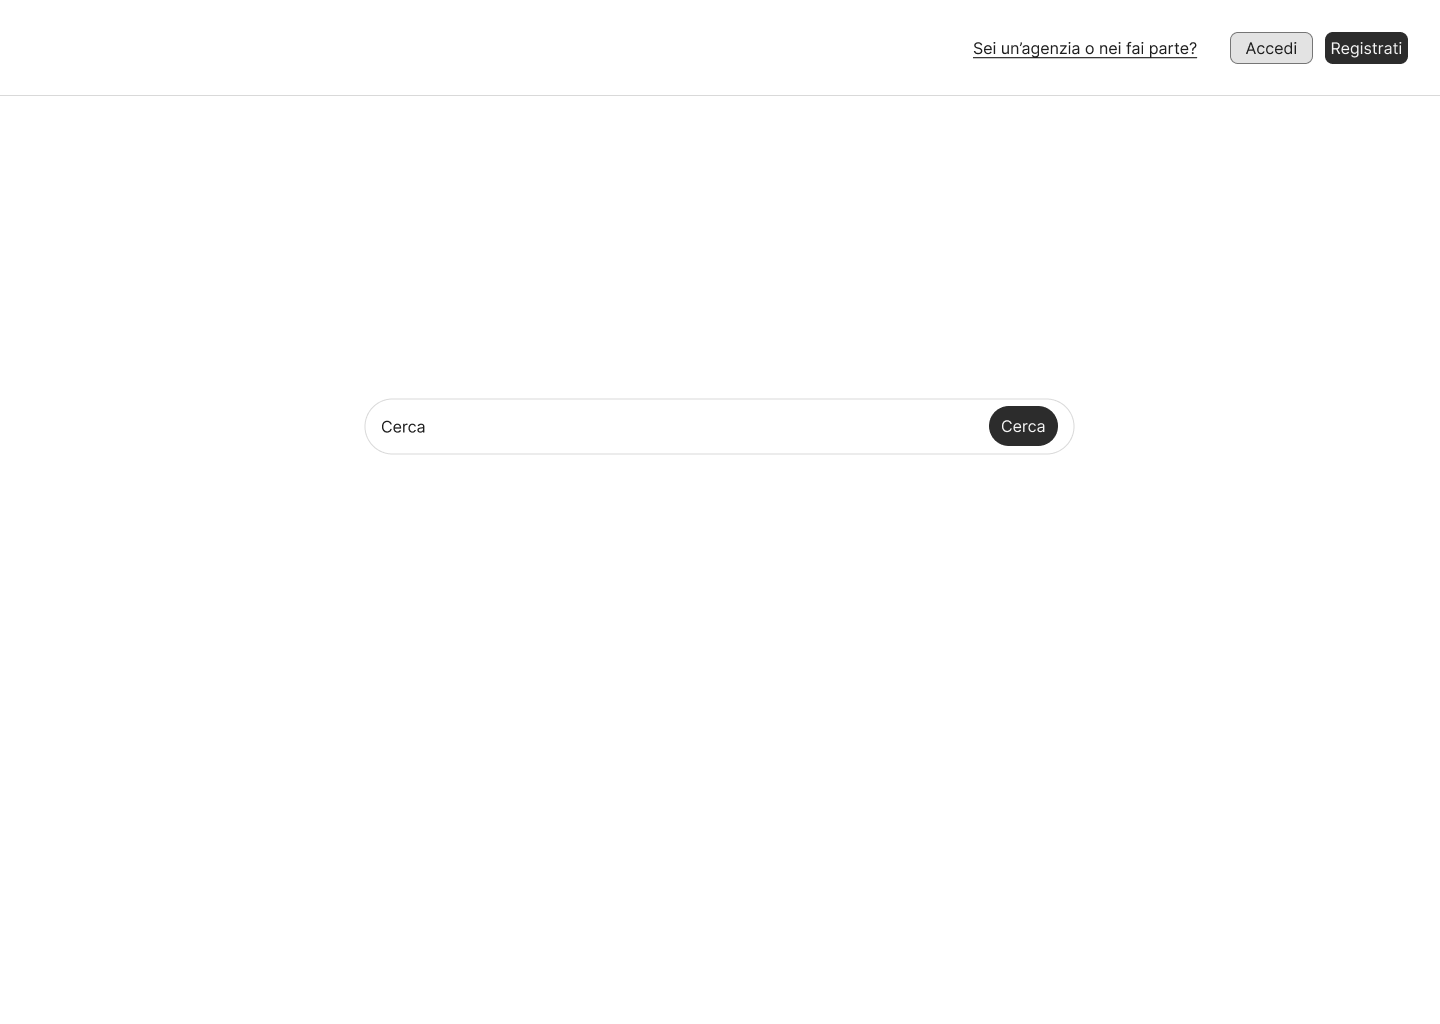
\includegraphics[width=\textwidth]{assets/mockups/ricerca-immobili/M-RI1.png}}
    \caption{M-RI1}
    \label{fig:M-RI1}
\end{figure}

\begin{figure}[h]
    \centering
    \fbox{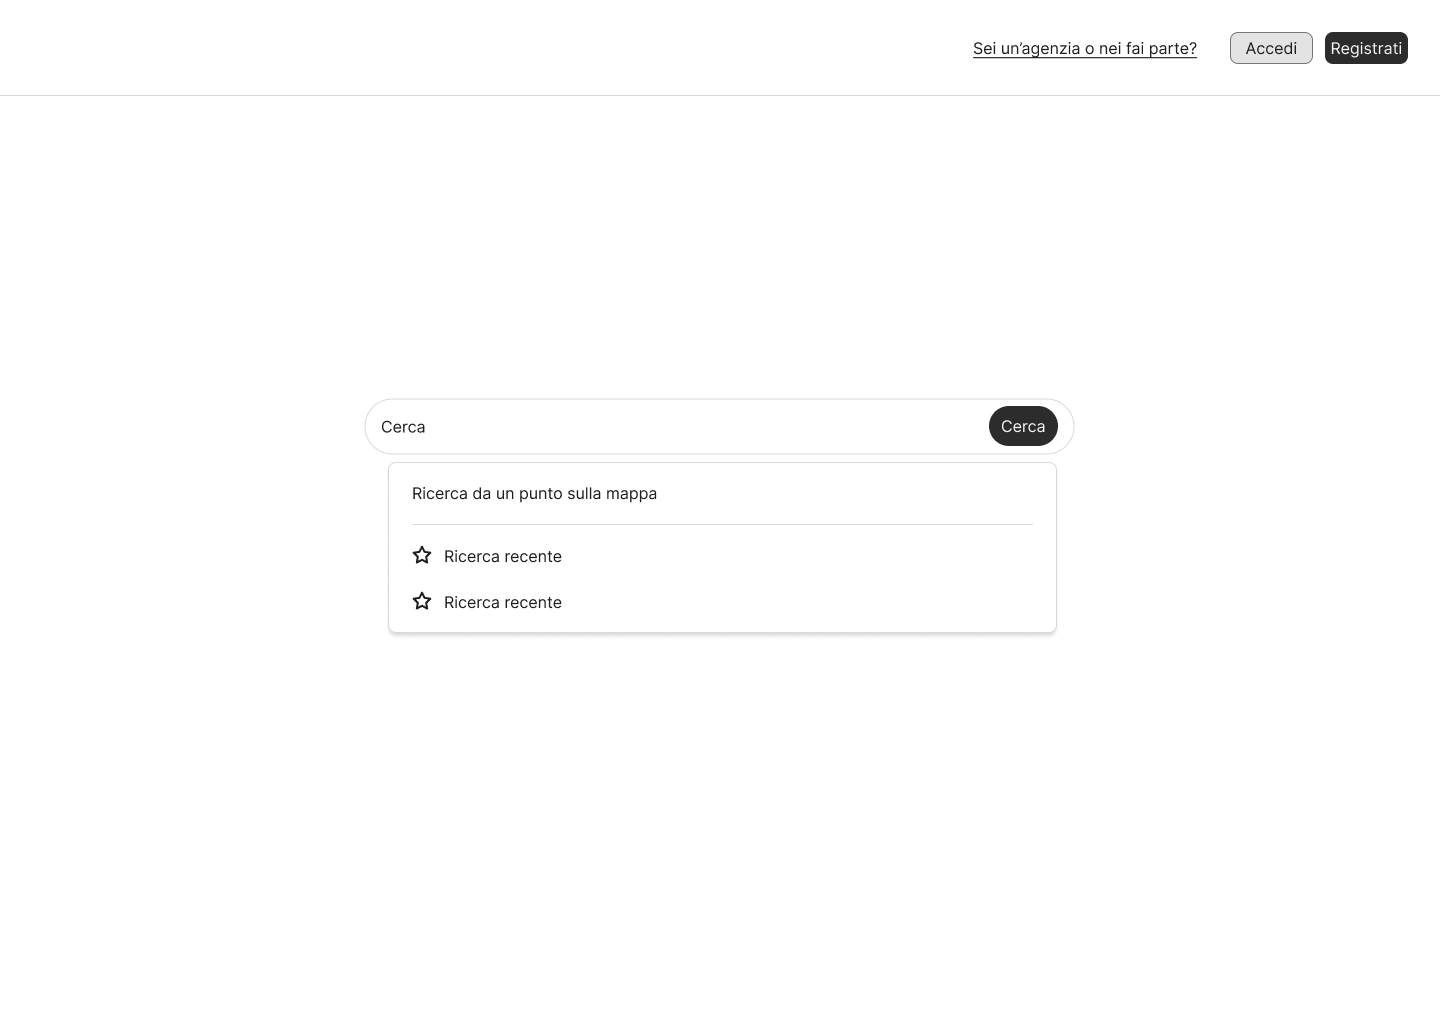
\includegraphics[width=\textwidth]{assets/mockups/ricerca-immobili/M-RI2.png}}
    \caption{M-RI2}
    \label{fig:M-RI2}
\end{figure}

\begin{figure}[h]
    \centering
    \fbox{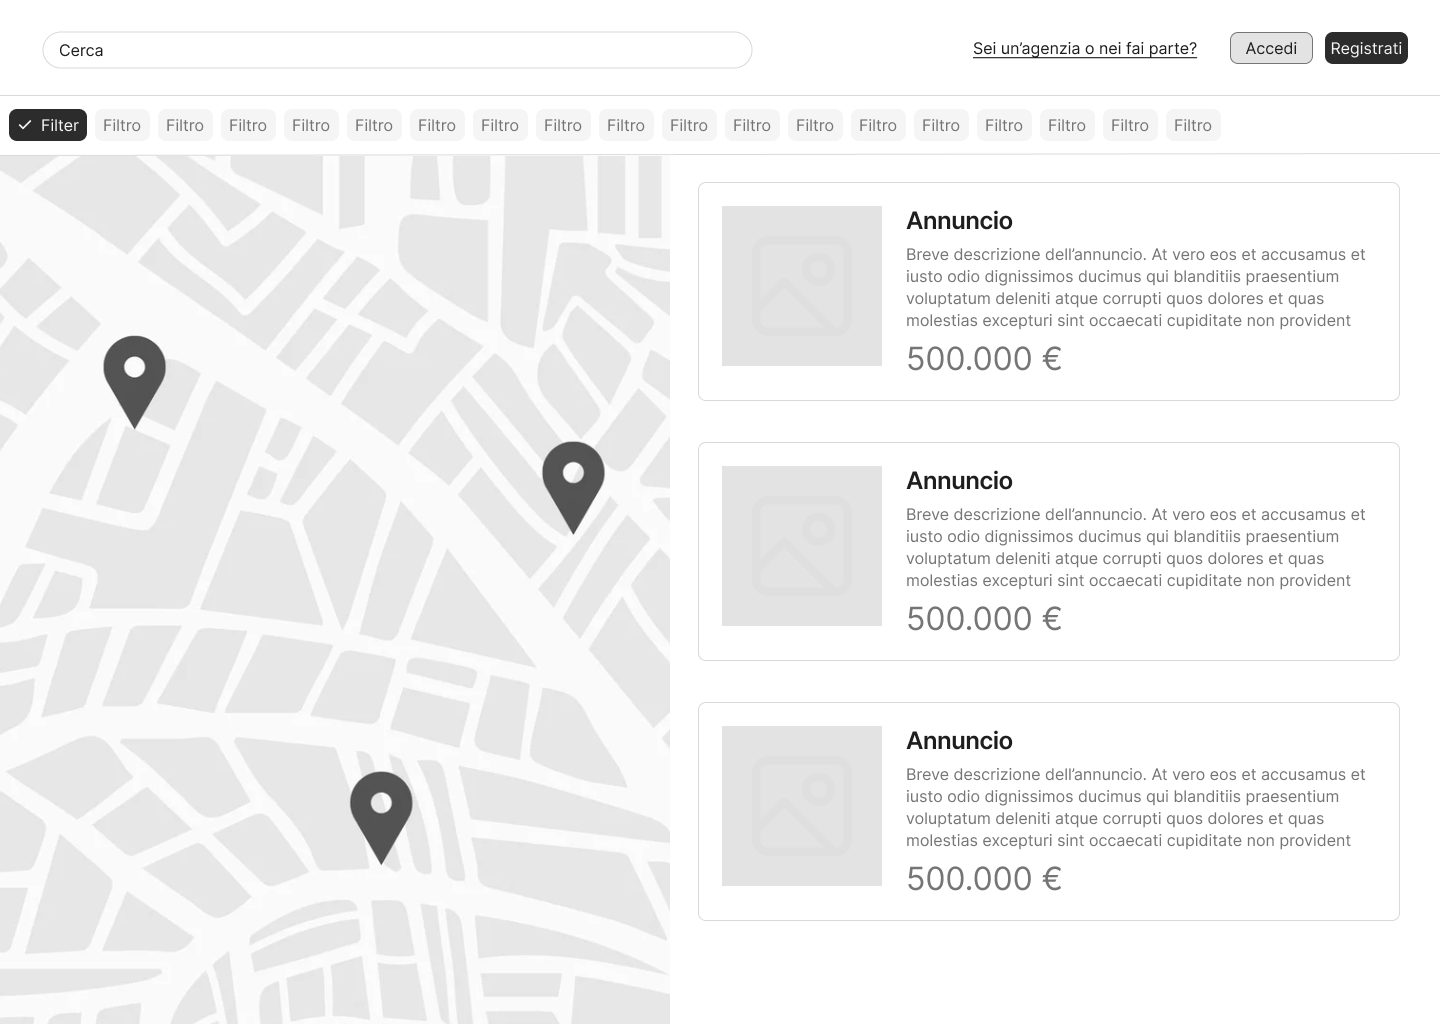
\includegraphics[width=\textwidth]{assets/mockups/ricerca-immobili/M-RI3.png}}
    \caption{M-RI3}
    \label{fig:M-RI3}
\end{figure}

\begin{figure}[h]
    \centering
    \fbox{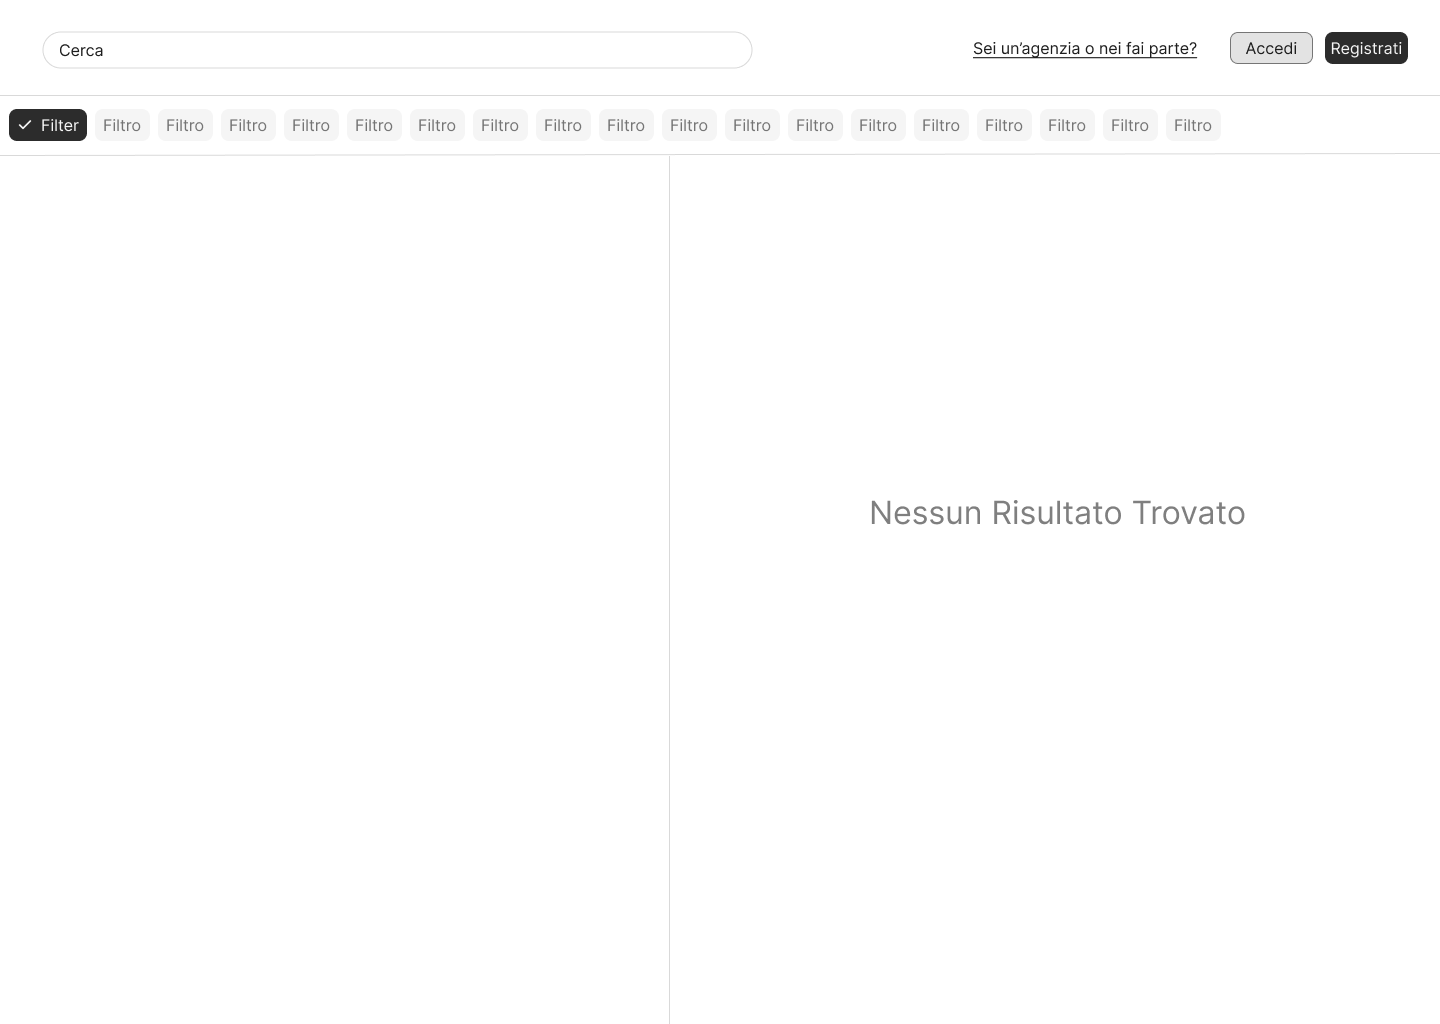
\includegraphics[width=\textwidth]{assets/mockups/ricerca-immobili/M-RI3bis.png}}
    \caption{M-RI3bis}
    \label{fig:M-RI3bis}
\end{figure}

\begin{figure}[h]
    \centering
    \fbox{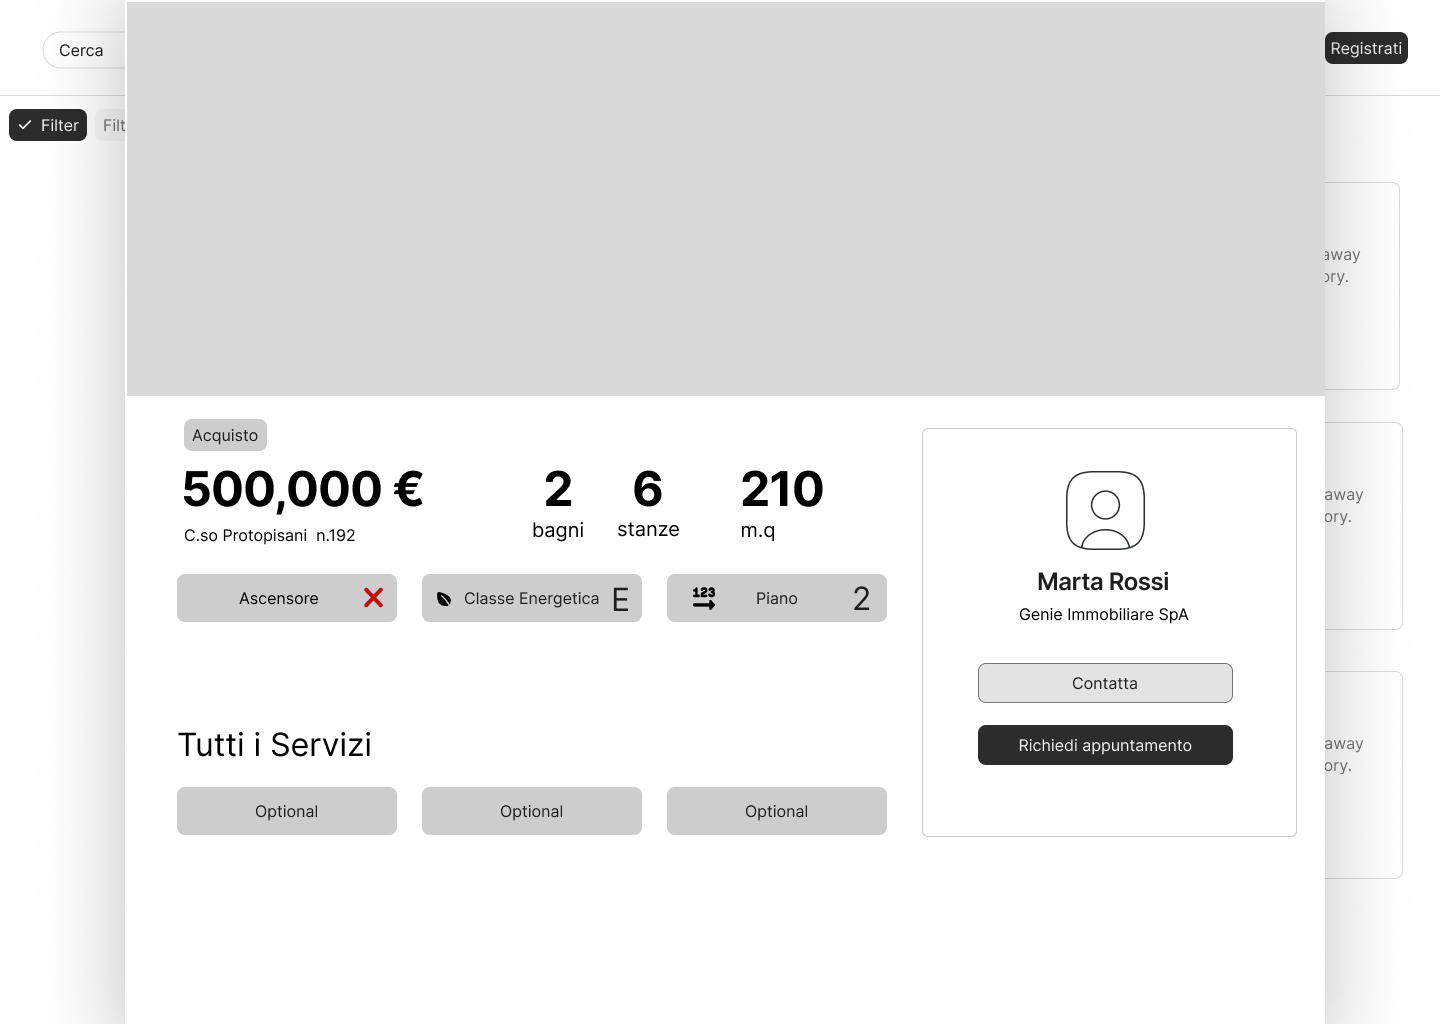
\includegraphics[width=\textwidth]{assets/mockups/ricerca-immobili/M-RI4.png}}
    \caption{M-RI4}
    \label{fig:M-RI4}
\end{figure}

\subsection{Fissa Appuntamento}
% Per tabelle che occupano più di una pagina:
%  longtblr al posto di tblr
\begin{longtblr}[
    caption = {Diagramma di Cockburn del caso d'uso \textit{Fissa Appuntamento}.}
]{
    column{1} = {3cm},
    column{2} = {0.8cm},
    column{3-5} = {3cm},
	vlines = {}, %per le cornici verticali
	hlines = {}, %per le cornici orizzontali
    % Merge delle righe/colonne:
    cell{1-7}{2} = {c = 4}{10cm, halign = l},
    cell{8}{1} = {r = 9}{valign = t},
    cell{17}{1} = {r = 3}{valign = t},
    cell{20}{1} = {r = 3}{valign = t},
    cell{23}{1} = {r = 3}{valign = t},
    cell{26}{2} = {c = 4}{10cm, halign = l}
}
USE CASE & Fissa appuntamento & & & \\
Goal in Context & Il Cliente vuole fissare un appuntamento con un Agente per la visione dell’immobile di interesse. & & & \\
Preconditions & Il Cliente deve essersi autenticato. & & & \\
Success End Condition & Il sistema tiene traccia della richiesta di appuntamento da parte del Cliente e la invia all’Agente. & & & \\
Fail End Condition & Il sistema non tiene traccia dell’attività non completata. & & & \\
Primary Actor & Cliente & & & \\
Trigger & Il Cliente preme il pulsante “Richiedi appuntamento” di \ref{fig:M-FA1}. & & & \\
Main Scenario   & Step & Cliente & Agente & System \\
 & 1 & Trigger action. & & \\
 & 2 & & & Mostra \ref{fig:M-FA2}. \\
 & 3 & Seleziona le sue preferenze. Clicca su Prosegui. & & \\
 & 4 & & & Mostra \ref{fig:M-FA3}. \\
 & 5 & Clicca su “Invia richiesta”. & & \\
 & 6 & & & Notifica al Cliente l'invio della richiesta. \\
 & 7 & & Accetta la richiesta. & \\
 & 8 & & & Notifica al Cliente la conferma dell’appuntamento e termina lo use case. \\
 
\pagebreak
Extension A & Step & Cliente & Agente & System \\
 & 3.a & Clicca su “Annulla”. & & \\
 & 4.a & & & Mostra \ref{fig:M-FA1} e termina use case.  \\
Extension B & Step & Cliente & Agente & System \\
 & 5.b & Clicca su “Annulla”. & & \\
 & 6.b & & & Torna allo step 2 del main scenario. \\
Extension C & Step & Cliente & Agente & System \\
 & 7.c & & Rifiuta la richiesta. & \\
 & 8.c & & & Invia al Cliente la notifica di rifiuto dell’appuntamento e termina lo use case. \\
Open Issues & & & & \\
\end{longtblr}
\begin{figure}[h]
    \centering
    \fbox{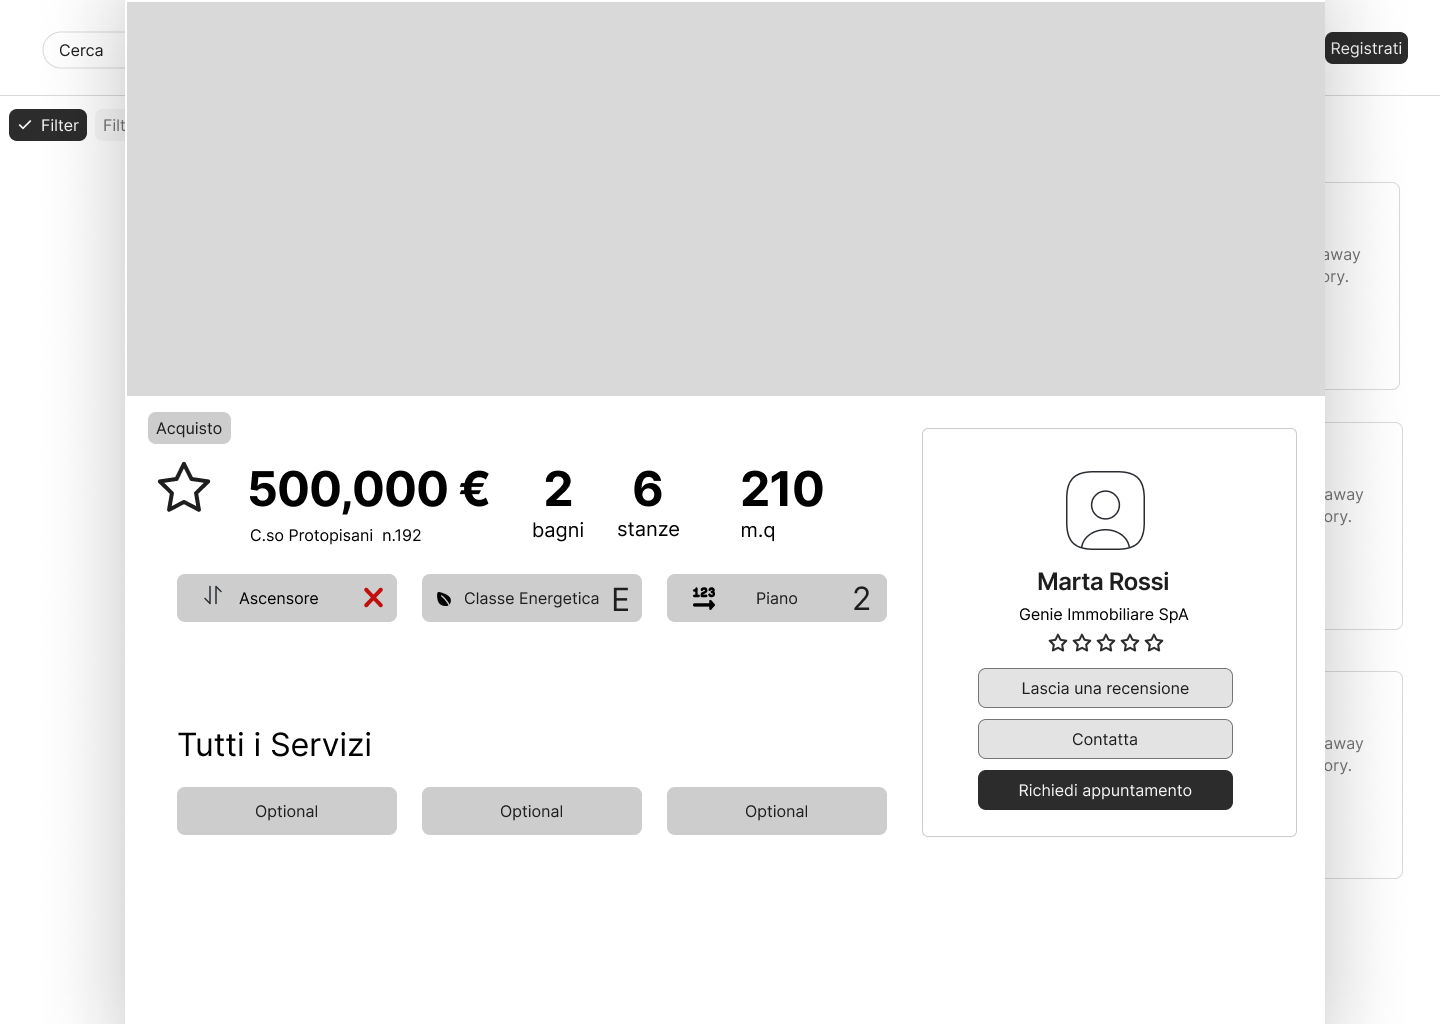
\includegraphics[width=\textwidth]{assets/mockups/fissa-appuntamento/M-FA1.png}}
    \caption{M-FA1}
    \label{fig:M-FA1}
\end{figure}
\begin{figure}[h]
    \centering
    \fbox{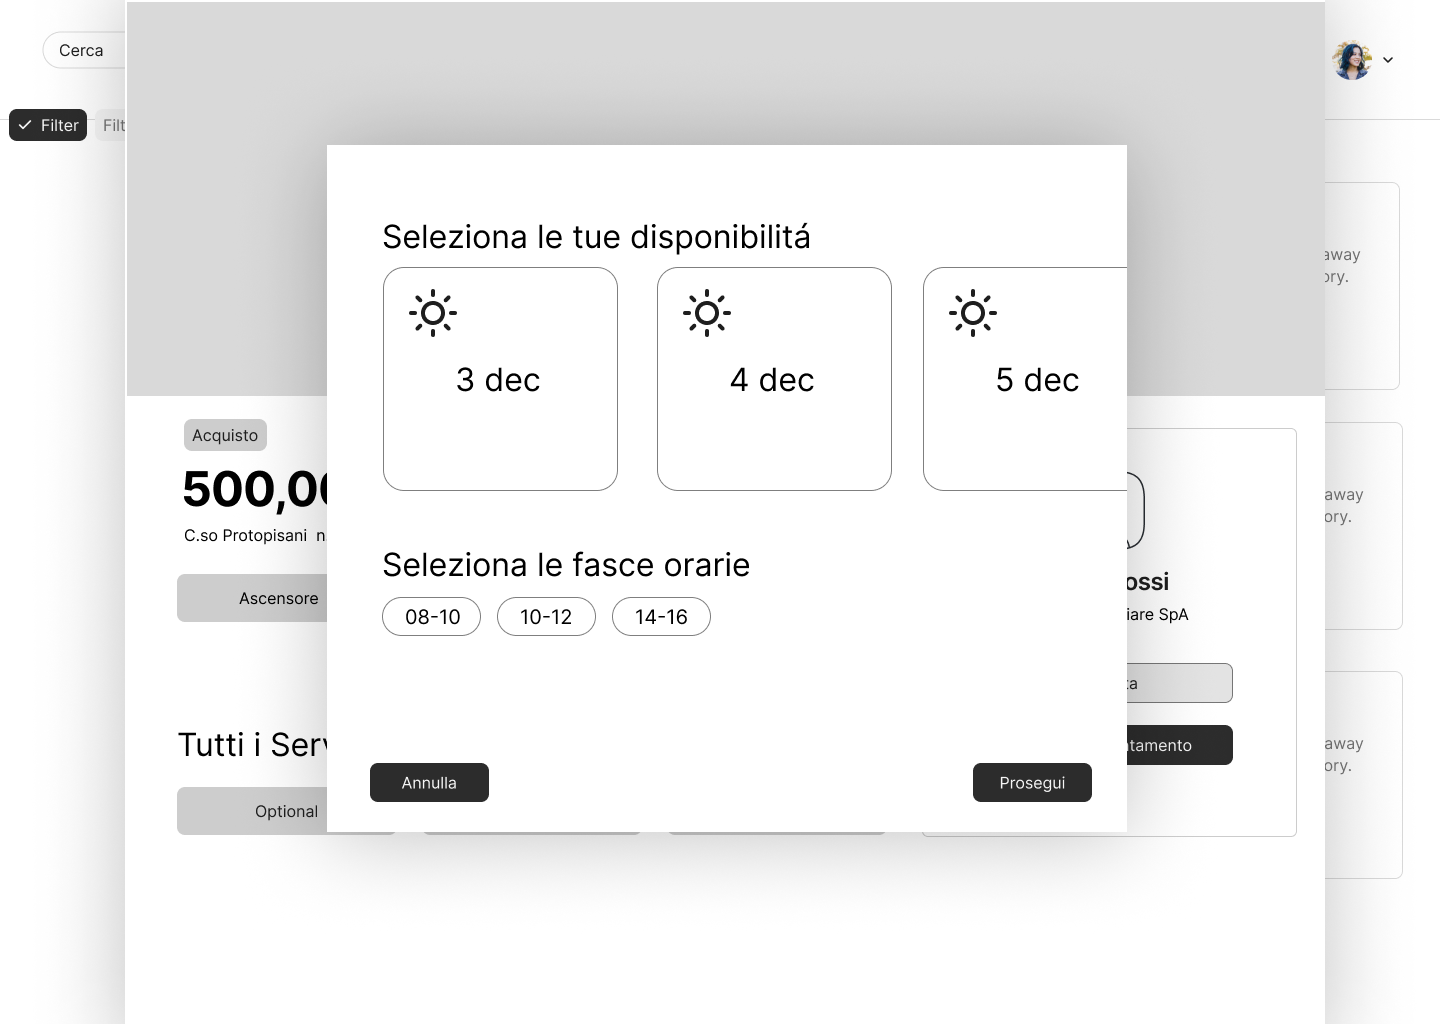
\includegraphics[width=\textwidth]{assets/mockups/fissa-appuntamento/M-FA2.png}}
    \caption{M-FA2}
    \label{fig:M-FA2}
\end{figure}
\begin{figure}[h]
    \centering
    \fbox{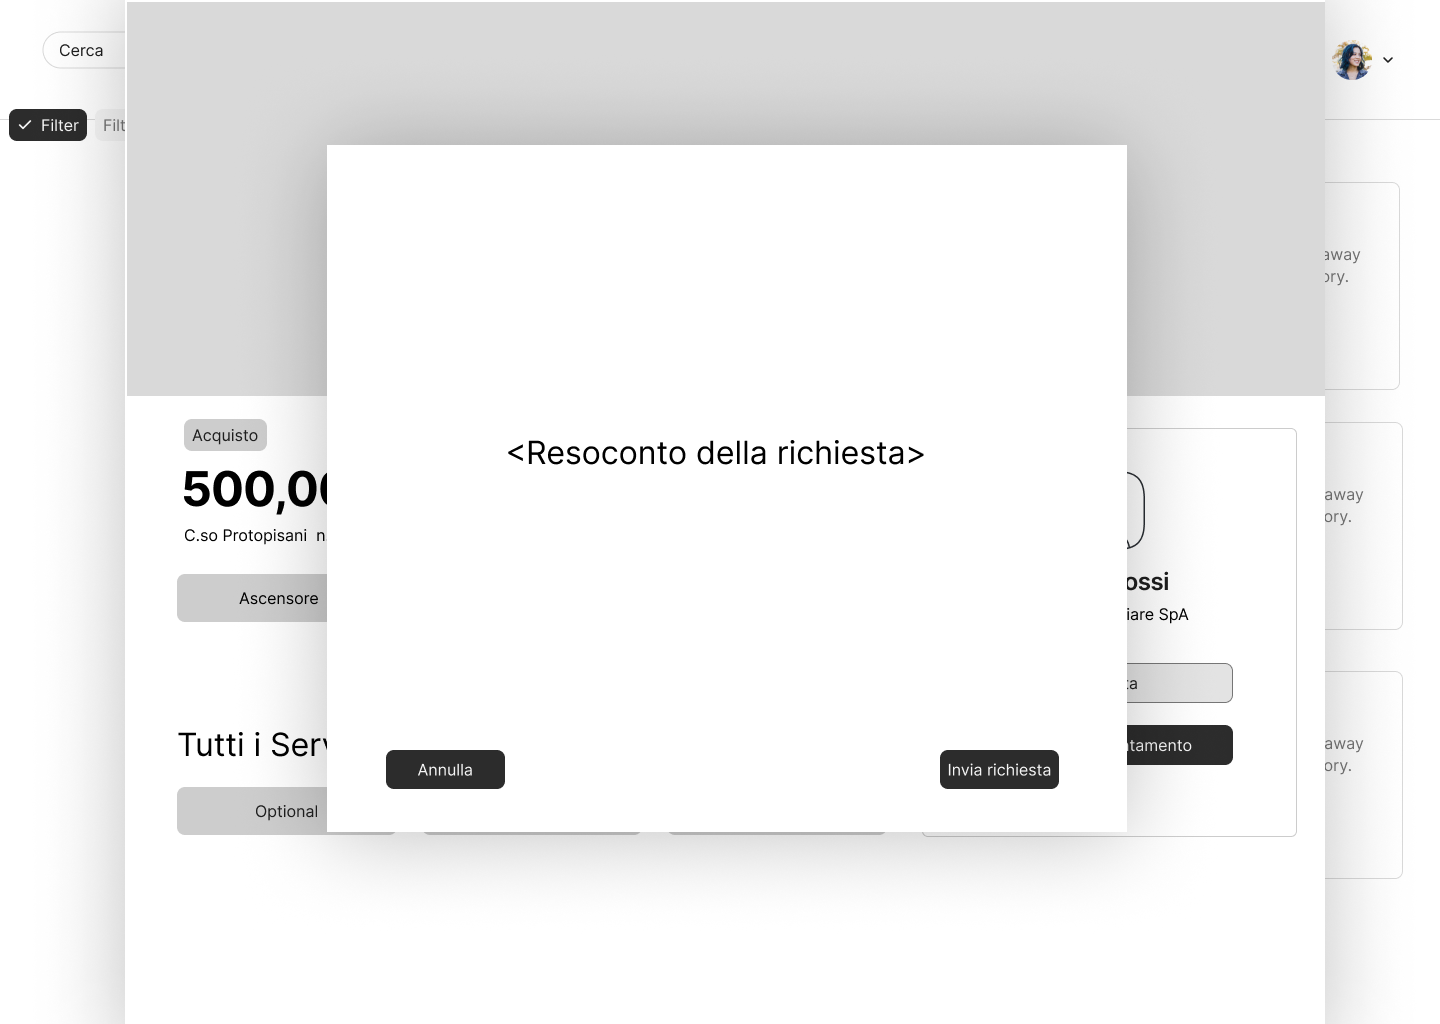
\includegraphics[width=\textwidth]{assets/mockups/fissa-appuntamento/M-FA3.png}}
    \caption{M-FA3}
    \label{fig:M-FA3}
\end{figure}

\subsection{Valuta Agente}
% Per tabelle che occupano più di una pagina:
%  longtblr al posto di tblr
\begin{longtblr}[
    caption = {Diagramma di Cockburn del caso d'uso Valuta Agente}
]{
    column{1} = {3cm},
    column{2} = {0.8cm},
    column{3-4} = {3cm},
	vlines = {}, %per le cornici verticali
	hlines = {}, %per le cornici orizzontali
    % Merge delle righe/colonne:
    cell{1-7}{2} = {c = 3}{10cm, halign = l},
    cell{8}{1} = {r = 5}{valign = t},
    cell{13}{1} = {r = 3}{valign = t},
    cell{16}{1} = {r = 3}{valign = t}
}
USE CASE & Valuta Agente & & \\
Goal in Context & Il Cliente vuole valutare la propria esperienza con un Agente & & \\
Preconditions & Il Cliente deve essere autenticato & & \\
Success End Condition & Il sistema tiene traccia della valutazione del Cliente & & \\
Fail End Condition & Il sistema non tiene traccia della valutazione del Cliente & & \\
Primary Actor & Cliente & & \\
Trigger & Il Cliente clicca sul pulsante "Aggiungi una recensione" della schermata \ref{fig:M-RI4} & & \\
Main Scenario & Step & Cliente & System   \\
 & 1 & Trigger & \\
 & 2 & & Mostra la schermata \ref{fig:M-VA1}\\
 & 3 & Inserisce una valutazione da una a cinque stelle e un commento. 
 Clicca poi sul pulsante "Invia Recensione". & \\
 & 4 & & Registra la recensione e termina caso d'uso. \\
 Extension A & Step & Cliente & System   \\
 & 3.a & Inserisce solo la valutazione, solo il commento, nessuna delle due. & \\
 & 4.a & & Mostra un messaggio di errore. Torna allo step 2 del main scenario. \\
Extension B & Step & Cliente & System   \\
 & 3.b & Clicca su un'altra parte dello schermo che non riguardi il popup per la recensione. & \\
 & 4.b & & Torna alla schermata precedente e termina use case. \\
\end{longtblr}

\subsection{Salva Annuncio}
% Per tabelle che occupano più di una pagina:
%  longtblr al posto di tblr
\begin{tblr}[
    caption = {Diagramma di Cockburn del caso d'uso Salva Annuncio}
]{
    column{1} = {3cm},
    column{2} = {0.8cm},
    column{3-4} = {3cm},
	vlines = {}, %per le cornici verticali
	hlines = {}, %per le cornici orizzontali
    % Merge delle righe/colonne:
    cell{1-7}{2} = {c = 3}{10cm, halign = l},
    cell{8}{1} = {r = 3}{valign = t}
}
USE CASE & Salva Annuncio & & \\
Goal in Context & Il Cliente vuole salvare l'annuncio trovato tra i preferiti
in modo tale da accedervi piú velocemente in futuro & & \\
Preconditions & Il Cliente deve essersi autenticato & & \\
Success End Condition & Il sistema aggiunge l'annuncio tra gli annunci salvati
del Cliente & & \\
Fail End Condition & Il sistema non aggiunge l'annuncio tra gli annunci salvati
del Cliente & & \\
Primary Actor & Cliente & & \\
Trigger & Il cliente clicca sul pulsante a forma di stella presente sull'annuncio
d'interesse, nella schermata \ref{fig:M-RI4} & & \\
Main Scenario   & Step & Cliente & System   \\
 & 1 & Trigger & \\
 & 2 & & Tiene traccia dell'aggiunta ai preferiti e termina use case. \\
\end{tblr}

\section{Requisiti non funzionali}
Il sistema deve soddisfare le seguenti qualitá:
\begin{list}{$\cdot$}{}
    \item availability, una scarsa availability é causa di perdita di 
    credibilitá e di utenza.
    \item adaptability, un utente deve poter accedere al servizio da tutti 
    i dispositivi possibili.
    \item performance efficiency, un software di ricerca lento è un software 
    morto in partenza.
    \item usability, l'utente deve poter utilizzare appieno il software già 
    dal primo utilizzo.
    \item scalability, una qualitá imprescindibile per un sistema utilizzato 
    da, potenzialmente, milioni di persone contemporaneamente.
    \item maintainability, la qualitá, interna, fondamentale per il successo 
    di un software. Essa, se presente, garantisce al team produttivitá nel tempo.
\end{list}

Il sistema deve rispettare le prassi e le tecnologie allo stato dell'arte per 
garantire security, soprattutto dal lato della confidentiality, in ottica di 
rispetto della privacy e della sicurezza dei dati personali dell'utente.

\section{Requisiti di dominio}
Ciascun annuncio deve possere le seguenti caratteristiche obbligatorie:
\begin{list}{$\cdot$}{}
    \item Tipologia dell'immobile. Valore selezionabile da elenco predefinito 
    (appartamento, villa, terreno, ecc.)
    \item Superficie. Valore numerico espresso in metri quadri ($m^2$).
    \item Numero di locali (non previsto per alcune tipologie di immobile).
    \item Numero di bagni (non previsto per alcune tipologie di immobile).
    \item Piano (non previsto per alcune tipologie di immobile).
    \item Prezzo/canone.
    \item Classe energetica conforme alla classificazione APE (da A4 a G).
    \item Indirizzo e coordinate geografiche.
    \item Comune.
    \item Provincia.
    \item Contatto di un agente immobiliare.
    \item Titolo annuncio.
\end{list}

Le caratteristiche obbligatorie degli annunci potranno essere aggiornate in 
funzione di modifiche normative o esigenze di mercato. Il sistema deve essere 
progettato per adattarsi flessibilmente a tali variazioni con impatto minimo 
sull'architettura complessiva.

\chapter{Design del sistema}

\section{Design Goals}
Il design di un sistema software deve essere svolto a valle di un'attenta 
analisi degli obiettivi di design, tradeoffs nell'ambito delle qualitá del 
software che rendano il software il piú adatto possibile per le sue ragioni 
di essere.

Il design del sistema deve essere costruito a partire dai requisiti non funzionali
descritti nel capitolo precedente.

\section{Design di alto livello}
Il sistema è suddiviso in due macro-componenti distribuite, comunicanti tramite 
rete:
\begin{list}{$\cdot$}{}
    \item Front-end. Il software che fornisce l'interfaccia con l'utente. Il front-end 
    interroga il back-end e restituisce le risposte che riceve da quest'ultimo.
    \item Back-end, detentore del Core, in cui viene gestita la logica di gestione delle 
    richieste e di manipolazione dei dati. Nel flusso di esecuzione, il Core è preceduto 
    da un Load Balancer, un middleware che gestisce il flusso di richieste per garantire 
    bilanciamento del carico tra le istanze del backend. I dati strutturati (entitá) sono 
    salvati su un DBMS, mentre i dati non strutturati (blob, immagini) sono salvati su un 
    Object Storage.
\end{list}

L'inserimento di una CDN (Content Delivery Network) é stato valutato e rimandato al 
futuro in quanto la geo-distribuzione non è, per adesso, obiettivo del sistema.

Sia front-end che back-end verranno descritti piú a fondo nelle sezioni successive.

\begin{figure}[H]
    \centering
    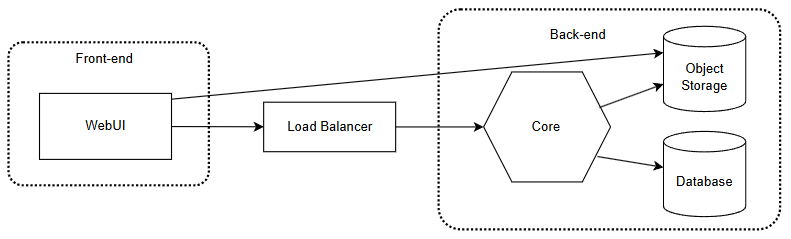
\includegraphics[width=\textwidth]{assets/diagrams/high-level-arch.png}
    \caption{L'architettura di alto livello}
    \label{fig:Architettura di alto livello}
\end{figure}

\begin{figure}[H]
    \centering
    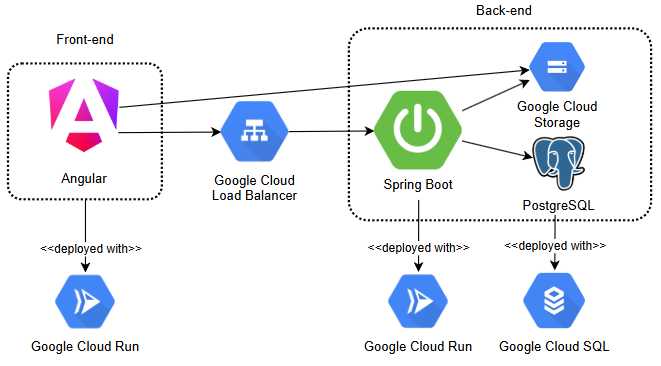
\includegraphics[width=\textwidth]{assets/diagrams/high-level-arch-tecnologies.png}
    \caption{L'architettura di alto livello, con tecnologie}
    \label{fig:Architettura di alto livello, con tecnologie}
\end{figure}

L'infrastruttura scelta per il deployment é Google Cloud, che garantisce availability 
di 99.95\% per i servizi di Run, SQL, Storage, per cui garantisce anche una durability 
ad undici 9.

Angular é stato scelto per implementare il front-end con una SPA (Single Page 
Application). La scelta di un'interfaccia web è figlia dell'obiettivo di alta 
adaptability.

Spring Boot é stato scelto per l'implementazione del core del sistema grazie al ridotto 
time-to-market che esso garantisce e alla sua affidabilitá dovuta al suo massiccio 
utilizzo nell'industria moderna. Spring Boot permette una facile integrazione di un 
potente ORM (Object Relational Mapping) come JPA (Java Persistence API).

PostgreSQL è stato scelto come DBMS per la sua efficienza e per il suo supporto nativo 
ai dati geografici (estensione PostGIS).

La scelta di un unico Cloud Provider permette una riduzione notevole della latenza nelle 
comunicazioni tra i componenti del sistema.

\section{Design del back-end}

\subsection{Persistenza dei dati}
Si presenta adesso lo schema per la persistenza dei dati.
Si é deciso, per alcune tabelle (Listing, User, Notification, Search) di definire
una struttura dotata di ereditarietá, per un'integrazione pulita con lo schema dei dati
del servizio Spring Boot. L'integrazione tra Spring Boot e il database é gestita da JPA.

É fornita ora una brevissima panoramica sulle possibili strategie per
l'implementazione di strutture gerarchiche basate sull'ereditarietá in un
DBMS relazionale.
\subsubsection{Ereditarietá in un DBMS relazionale}
I DBMS relazionali non supportano nativamente l'ereditarietá per come essa é nota
ai conoscitori dei linguaggi object-oriented. Tuttavia, é possibile applicare dei
noti pattern per sopperire a questa limitazione:
\begin{list}{$\cdot$}{}
    \item Single Table: si memorizzano tutti gli attributi di tutte le 
    classi (superclasse e sottoclassi) in un'unica tabella. Include un campo discriminatore 
    che indica il tipo specifico di ogni record.
    \item Joined Table: si crea crea una tabella separata per ogni classe nella gerarchia. 
    La tabella della sottoclasse contiene solo gli attributi specifici e una chiave esterna 
    che punta alla tabella della superclasse.
    \item Table Per Class: si crea una tabella separata e completa per ogni sottoclasse, 
    includendo sia gli attributi ereditati dalla superclasse che quelli specifici.
\end{list}

\begin{table}[H]
    \centering
    \begin{tabularx}{\textwidth}{|X|X|X|X|}
    \hline
    \textbf{Aspetto} & \textbf{Single Table} & \textbf{Joined Table} & \textbf{Table Per Class} \\
    \hline
    \textbf{Spreco di dati} & 
    Alto. Tutti gli attributi di tutte le sottoclassi sono memorizzati in un'unica tabella, con molti valori NULL per gli attributi non pertinenti alla classe specifica. & 
    Basso. Ogni tabella contiene solo gli attributi specifici della classe corrispondente, minimizzando lo spazio inutilizzato. & 
    Medio. Ciascuna tabella è completa ma si ha duplicazione degli attributi della superclasse in ogni tabella delle sottoclassi. \\
    \hline
    \textbf{Velocità di lettura} & 
    Alta. Nessun JOIN necessario per recuperare un oggetto completo, le query sono generalmente più veloci. & 
    Media/Bassa. Richiede JOIN tra le tabelle della gerarchia per ricostruire oggetti completi, penalizzando le performance con gerarchie profonde. & 
    Alta per singole sottoclassi. Bassa per query polimorfiche sulla superclasse che richiedono UNION di tutte le tabelle delle sottoclassi. \\
    \hline
    \textbf{Velocità di inserimento} & 
    Alta. Un singolo INSERT in un'unica tabella. & 
    Media. Richiede INSERT multipli (uno nella tabella della superclasse e uno nella tabella della sottoclasse). & 
    Alta. Un singolo INSERT in una tabella concreta. \\
    \hline
    \textbf{Velocità di aggiornamento} & 
    Alta. UPDATE su un'unica tabella. & 
    Media. Può richiedere UPDATE su più tabelle se si modificano attributi ereditati. & 
    Alta per attributi specifici, ma richiede aggiornamenti multipli se si modificano gli stessi attributi in classi differenti. \\
    \hline
    \end{tabularx}
    \caption{Confronto tra strategie di implementazione dell'ereditarietà in JPA}
    \label{tab:inheritance-comparison}
    \end{table}

Alla luce di questa disamina, si é deciso di:
\begin{list}{$\cdot$}{}
    \item applicare la strategia Joined Table per la gerarchia con radice la tabella USER, in quanto
    is prevede che il numero di utenti di tipo CUSTOMER sia maggiore 
    degli altri di diversi ordini di grandezza.
    \item applicare la strategia Single Table per le gerarchie di SEARCH,
    LISTING: HOUSE é, secondo le stime, la sottoclasse che
    avrá piú istanze, di gran lunga sulle altre.
    \item applicare la strategia Single Table per la gerarchia di NOTIFICATION:
    i campi nulli sono pochi. Inoltre, la tabella NOTIFICATION é una mera tabella
    di outbox (si parlerá di seguito dell'outbox pattern), per cui le sue righe sono
    destinate ad essere eliminate in tempi brevi.
\end{list}

Si motiva adesso l'esistenza della tabella NOTIFICATION.
\subsubsection{L'OUTBOX Pattern}
Il pattern Outbox rappresenta una soluzione elegante al problema della comunicazione affidabile 
tra servizi distribuiti, specialmente in contesti in cui la coerenza dei dati é fondamentale.
Nel nostro caso, non parliamo di coerenza di dati, ma semplicemente di affidabilitá di comunicazione:
una notifica persa é potenzialmente un grave problema nell'esperienza degli utenti: si pensi al caso 
in cui un agente accetti una richiesta di visita, ma la notifica non arrivi al cliente.

L'idea alla base è semplice: sfruttare le proprietá ACID di un DBMS (tipicamente relazionale) per 
inserire un evento e la comunicazione di esso all'interno della stessa transazione, inserendo la 
comunicazione in una tabella di OUTBOX.
Nel nostro caso, la tabella NOTIFICATION é una tabella di OUTBOX, da cui poi il sistema
potrá attingere per inviare le comunicazioni. Una volta consumate, le comunicazioni sono
rimosse dalla tabella.

\begin{figure}[H]
    \centering
    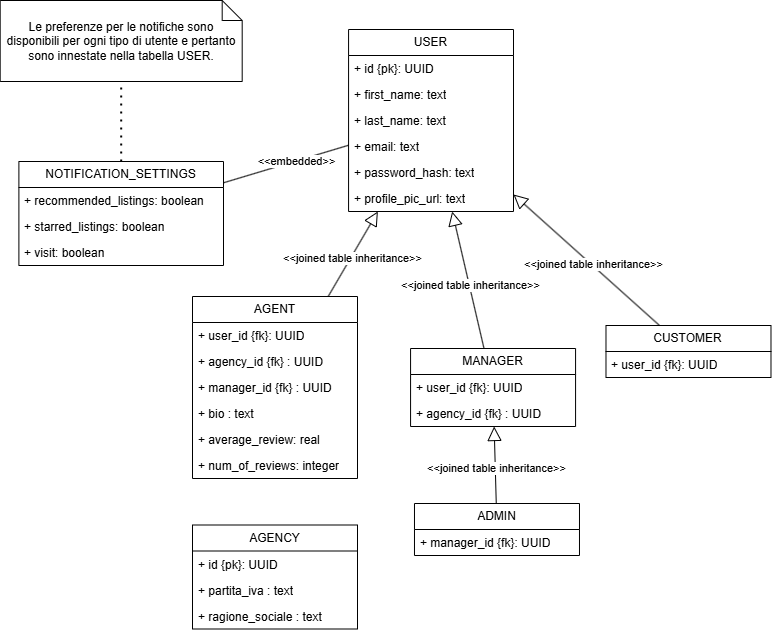
\includegraphics[width=\textwidth]{assets/diagrams/db-scheme/users.png}
    \caption{Lo schema di persistenza degli utenti.}
    \label{fig:Schema di persistenza degli utenti}
\end{figure}

\begin{figure}[H]
    \centering
    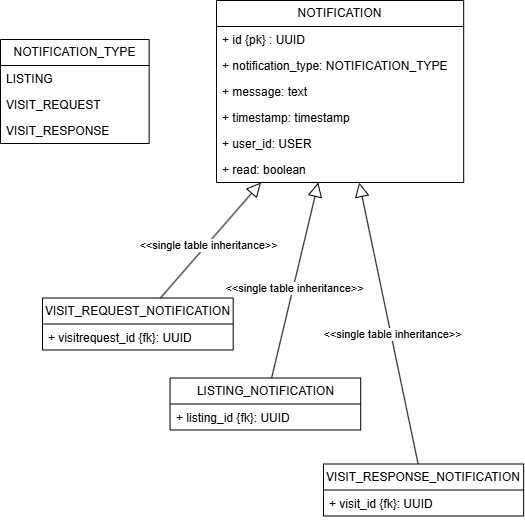
\includegraphics[width=\textwidth]{assets/diagrams/db-scheme/notification.png}
    \caption{Lo schema di persistenza delle notifiche.}
    \label{fig:Schema di persistenza delle notifiche}
\end{figure}

\begin{figure}[H]
    \centering
    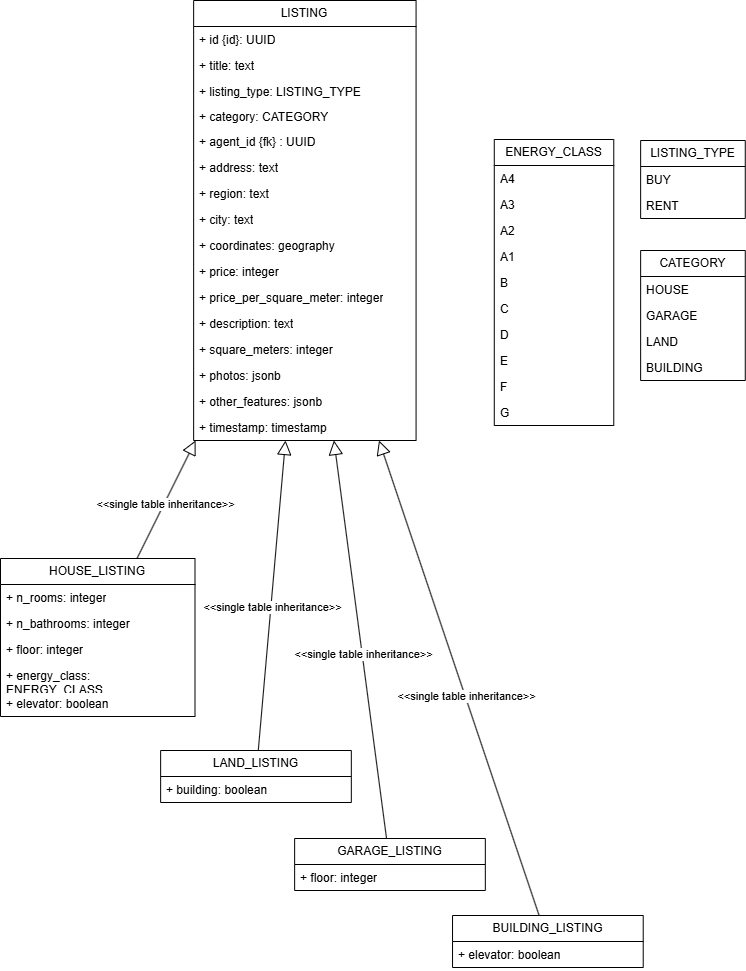
\includegraphics[width=\textwidth]{assets/diagrams/db-scheme/listing.png}
    \caption{Lo schema di persistenza degli annunci.}
    \label{fig:Schema di persistenza degli annunci}
\end{figure}

\begin{figure}[H]
    \centering
    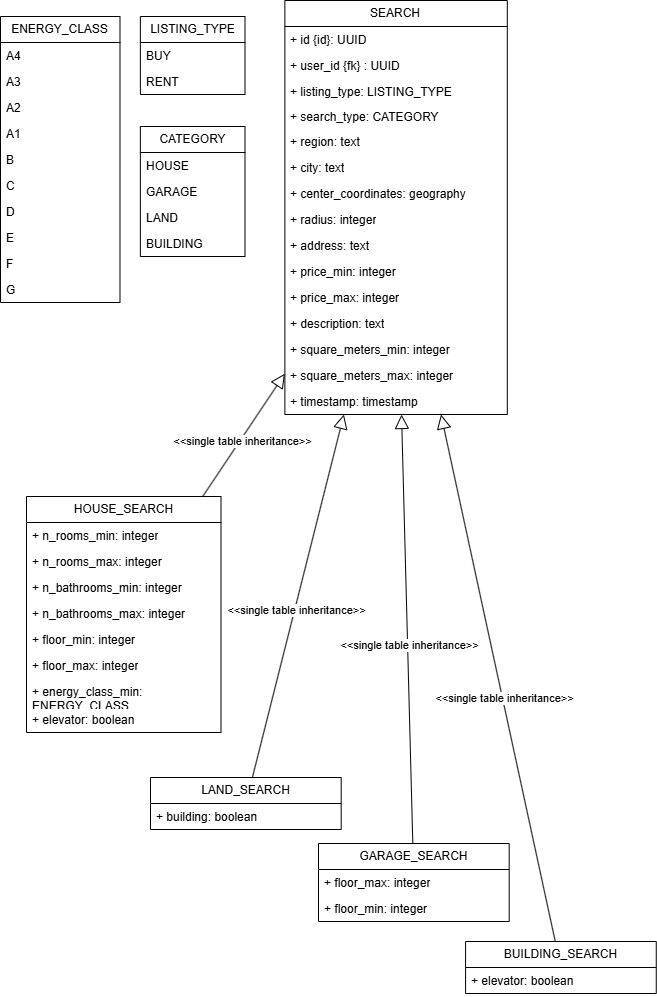
\includegraphics[width=\textwidth]{assets/diagrams/db-scheme/search.png}
    \caption{Lo schema di persistenza delle ricerche effettuate dagli utenti.}
    \label{fig:Schema di persistenza delle ricerche effettuate dagli utenti}
\end{figure}

\subsection{L'architettura esagonale}
La scelta di un framework opinionated come Spring Boot impone un’architettura ben precisa: 
l'architettura esagonale, anche detta port-and-adapters, formalizzata da A. Cockburn.

L’obiettivo di questa architettura é rendere il cosiddetto core facilmente testabile, 
manutenibile e molto agile di fronte a cambiamenti ed estensioni, permettendo di non 
stravolgere la codebase.

Per ottenere ciò, l’architettura esagonale definisce un confine netto tra il core e 
le estensioni, chiamate porte, che definiscono un contratto tra il core ed il componente 
esterno che fornisce l’estensione. Tale componente esterno é chiamato adapter.
Bisogna fare un distinguo tra porte in entrata e porte in uscita:
\begin{list}{$\cdot$}{}
    \item porte in entrata, spesso chiamate Service come nel caso di Spring, sono spesso 
    mappate a use case e definiscono possibili microservizi.
    \item porte in uscita sono interfacce che definiscono come il core puó utilizzare 
    un componente esterno.
\end{list}

Tale distinguo si riflette sugli adapter:
\begin{list}{$\cdot$}{}
    \item adapter in entrata, spesso chiamati Controller come nel caso di Spring, 
    usano le porte in entrata.
    \item adapter in uscita implementano le porte in uscita.
\end{list}

Sia le porte che gli adapter per la persistenza dei dati sono spesso chiamate Repository, 
come nel caso di Spring.

L’architettura esagonale: 
\begin{list}{$\cdot$}{}
    \item permette un testing efficace del core grazie alla dependency injection 
    alla base: il mocking delle dipendenze è molto semplificato.
    \item facilita l’aggiunta di nuove feature: si definisce una porta e la si 
    adatta con una tecnologia specifica.
    \item permette una migrazione naturale ad architetture piú modulari dal punto 
    di vista del deployment, come modular monolith e microservizi.
\end{list}

\subsection{Diagramma dei package}
Vengono presentati adesso i package che compongono il software.
\begin{list}{$\cdot$}{}
    \item auth: al suo interno é definita la logica di autenticazione del sistema ed
    e le operazioni su generici utenti. Viene impiegato al suo interno Spring Security,
    il modulo di Spring per la gestione della sicurezza.
    \item customer: al suo interno é definita la logica per la gestione
    dei clienti.
    \item agency: al suo interno é definita la logica per la gestione
    dell'agenzia e delle figure che la compongono: amministratore, gestori, agenti.
    \item listing: contiene la logica di creazione, gestione, ricerca di annunci.
    \item visit: contiene la logica per quanto concerne le richieste di visita e 
    le visite.
    \item agentreview: al suo interno vi é la logica di creazione e visualizzazione di 
    valutazioni degli agenti.
    \item starredlisting: contiene la logica della funzionalitá secondo cui
    un utente puó inserire tra i preferiti un annuncio.
    \item notification: definisce la logica di creazione ed invio delle
    notifiche.
\end{list}

\begin{figure}[H]
    \centering
    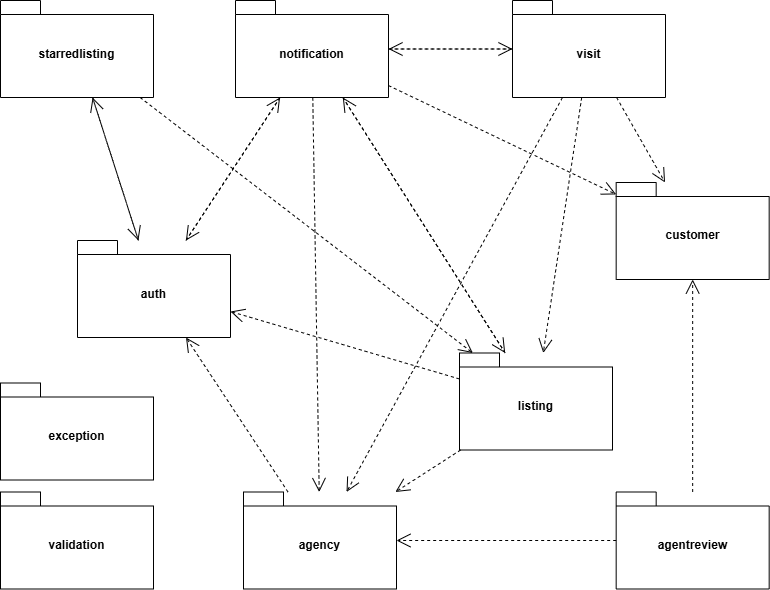
\includegraphics[width=\textwidth]{assets/diagrams/class-diagram/package.png}
    \caption{Il diagramma dei package.}
    \label{fig:Diagramma dei package}
\end{figure}

\begin{figure}[H]
    \centering
    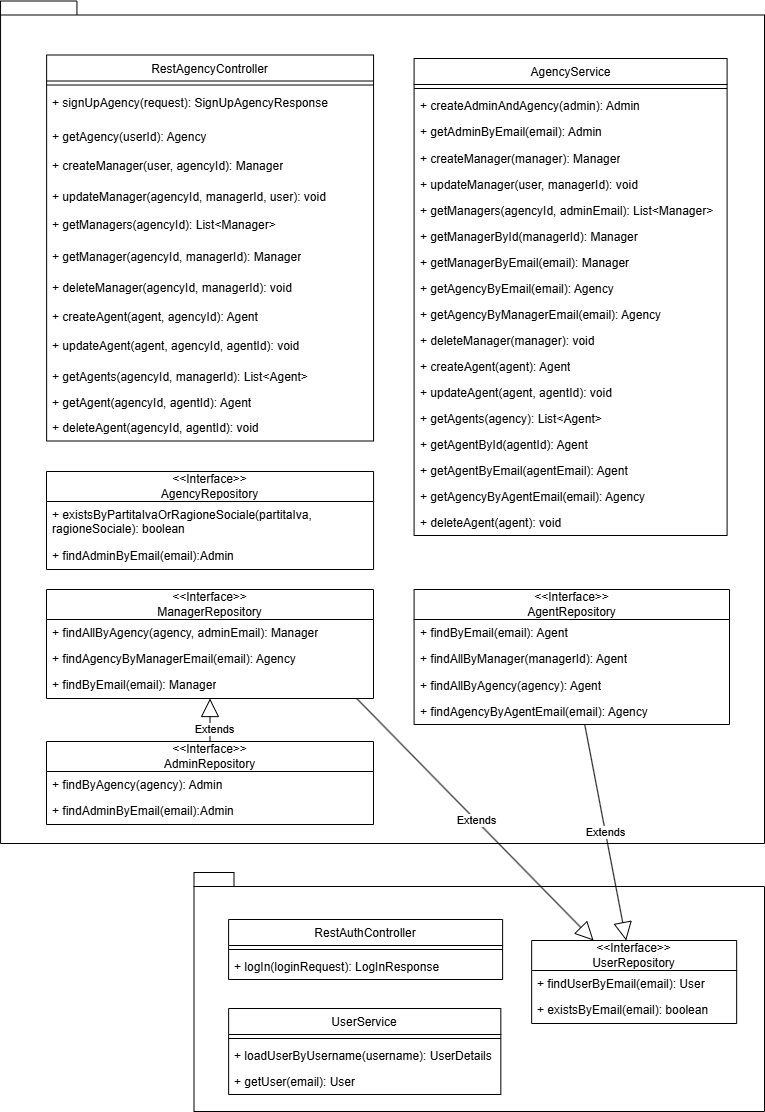
\includegraphics[width=\textwidth]{assets/diagrams/class-diagram/class-diagram-1.png}
    \caption{Parte del diagramma delle classi.}
    \label{fig:Parte 1 del diagramma delle classi}
\end{figure}

\begin{figure}[H]
    \centering
    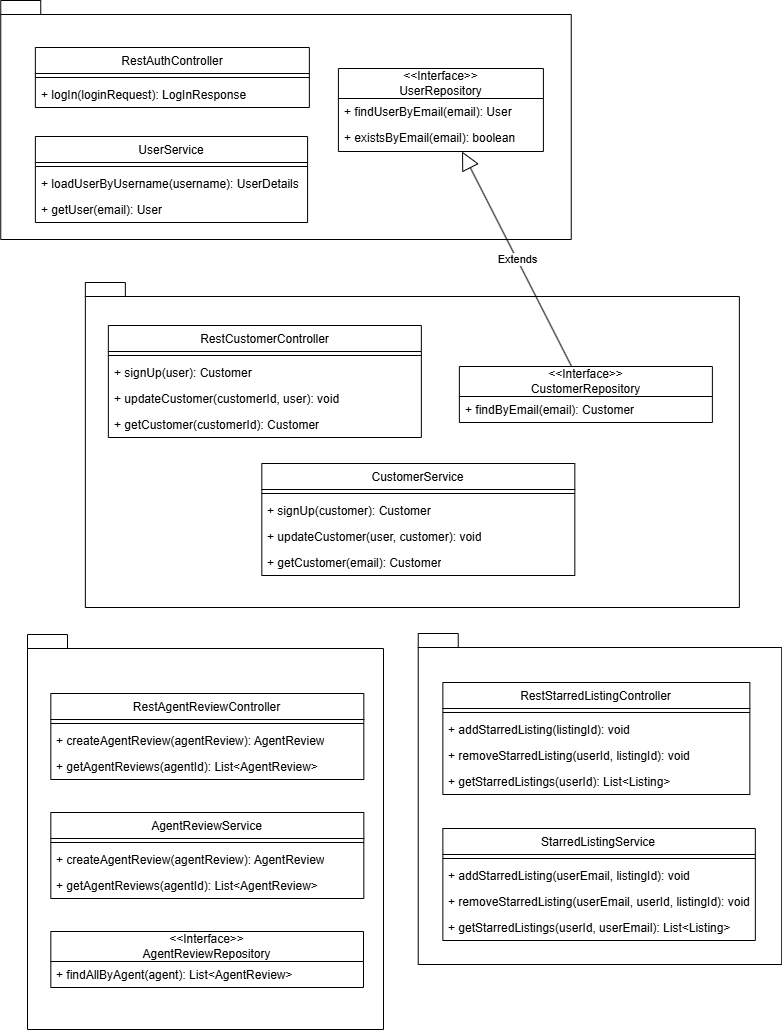
\includegraphics[width=\textwidth]{assets/diagrams/class-diagram/class-diagram-2.png}
    \caption{Parte del diagramma delle classi.}
    \label{fig:Parte 2 del diagramma delle classi}
\end{figure}

\begin{figure}[H]
    \centering
    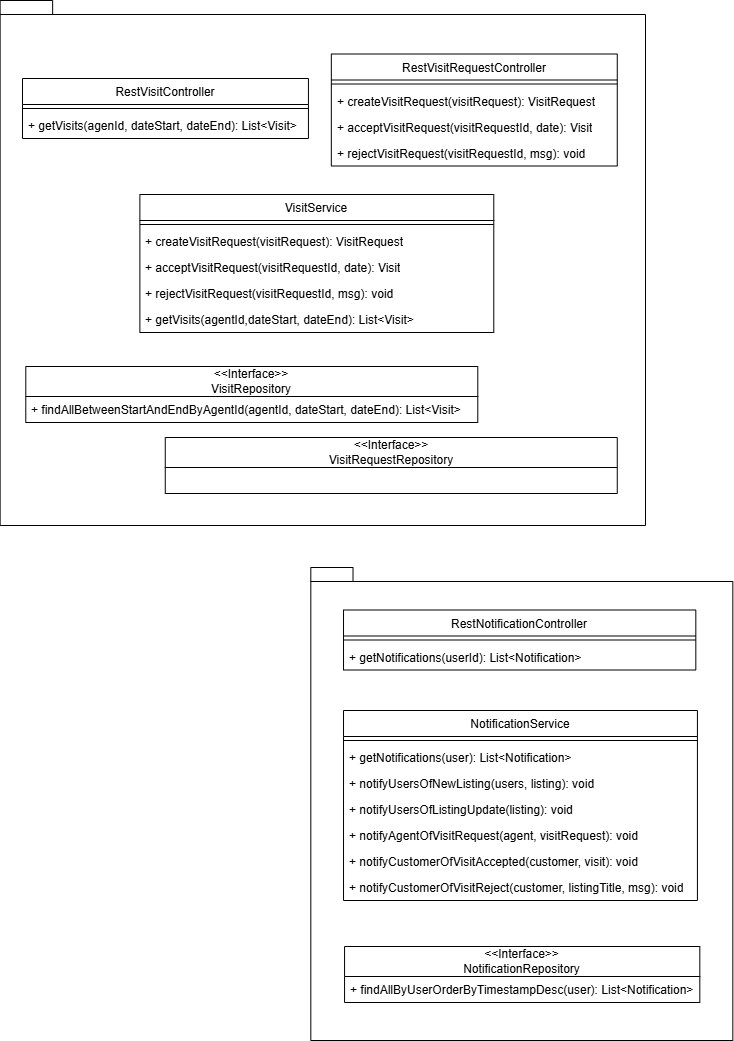
\includegraphics[width=\textwidth]{assets/diagrams/class-diagram/class-diagram-3.png}
    \caption{Parte del diagramma delle classi.}
    \label{fig:Parte 3 del diagramma delle classi}
\end{figure}

\begin{figure}[H]
    \centering
    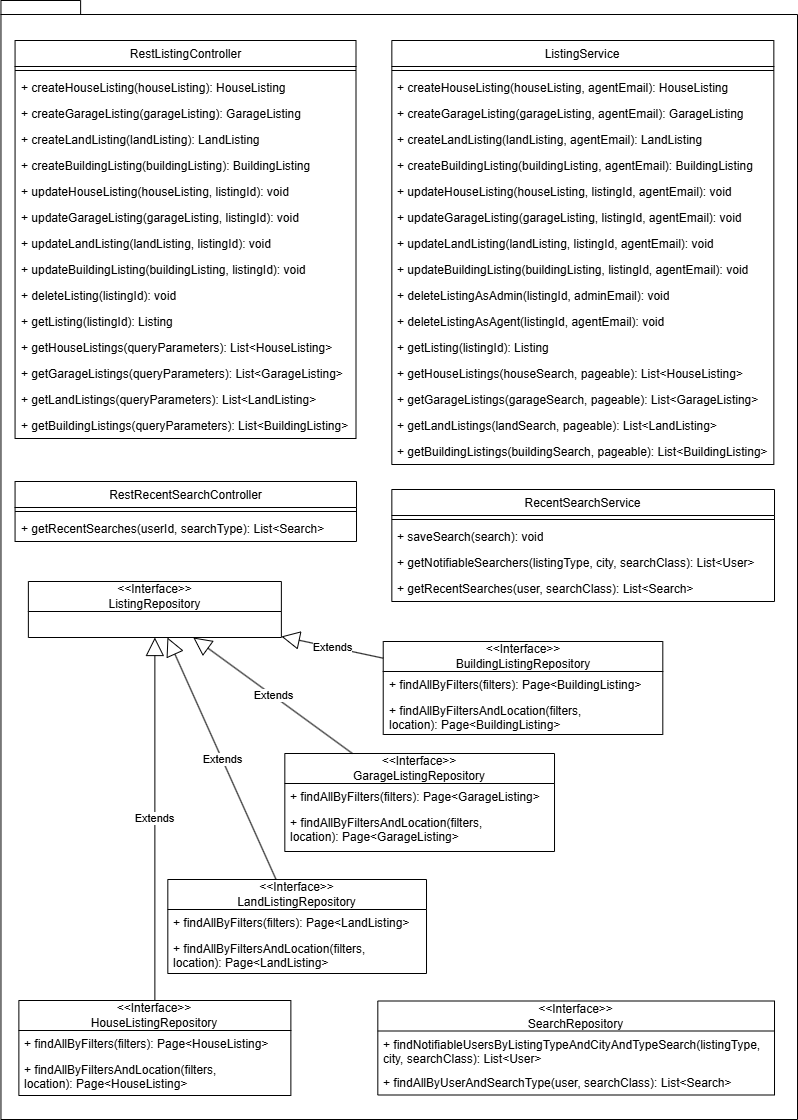
\includegraphics[width=\textwidth]{assets/diagrams/class-diagram/class-diagram-4.png}
    \caption{Parte del diagramma delle classi.}
    \label{fig:Parte 4 del diagramma delle classi}
\end{figure}

\subsection{Diagrammi di sequenza}
Vengono adesso documentati alcuni casi d'uso tramite diagramma di sequenza.

\begin{figure}[H]
    \adjustbox{width=1.4\textwidth,center}{
        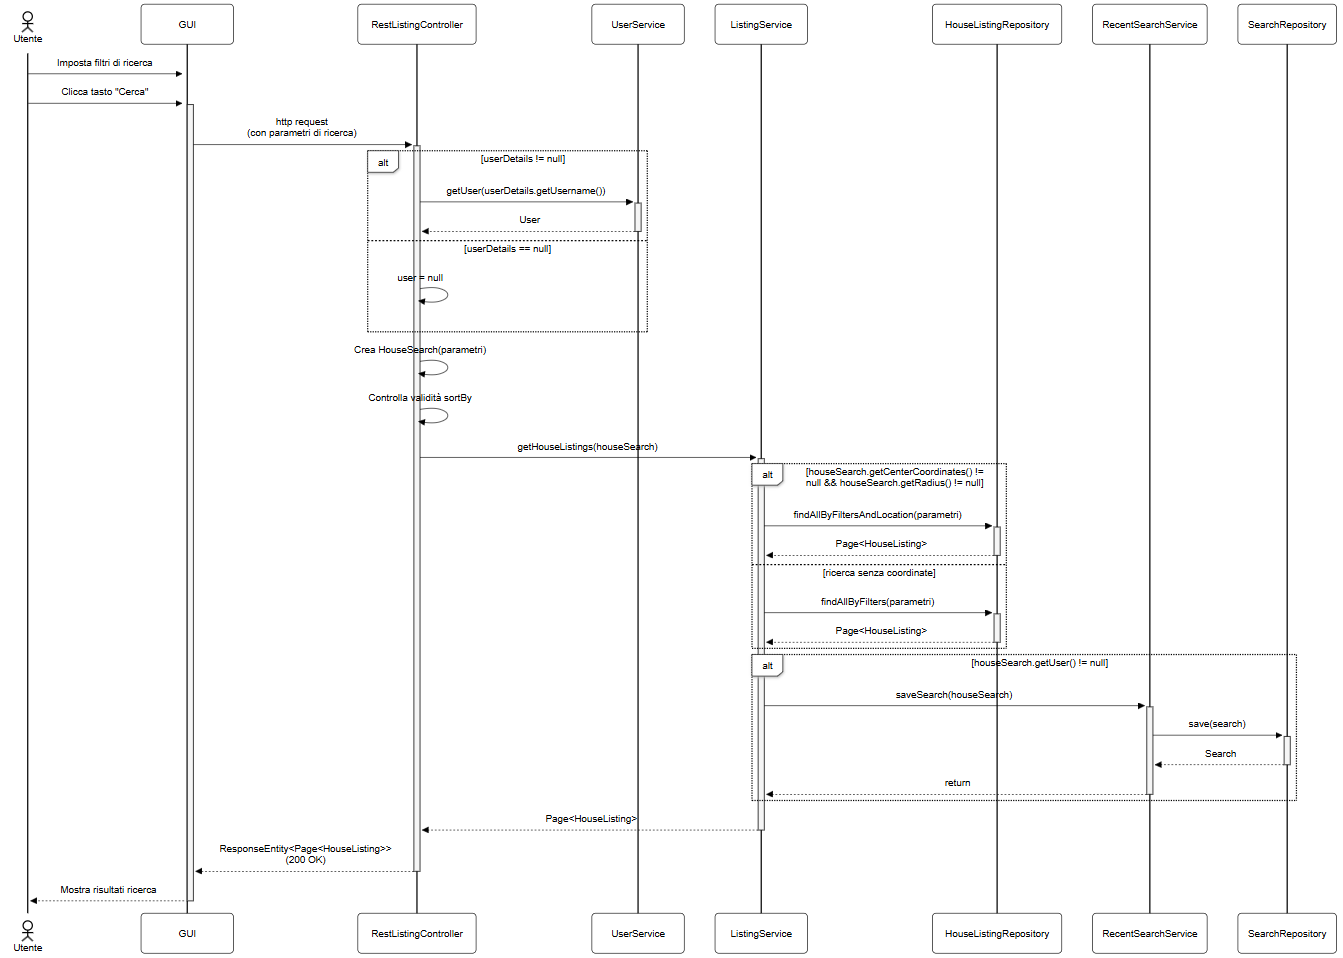
\includegraphics{assets/diagrams/sequence/ricerca-immobili.png}
    }
    \caption{Diagramma di sequenza del caso d'uso Ricerca Immobili.}
    \label{fig:Diagramma di sequenza del caso d'uso Ricerca Immobili}
\end{figure}

\begin{figure}[H]
    \adjustbox{width=1.4\textwidth,center}{
        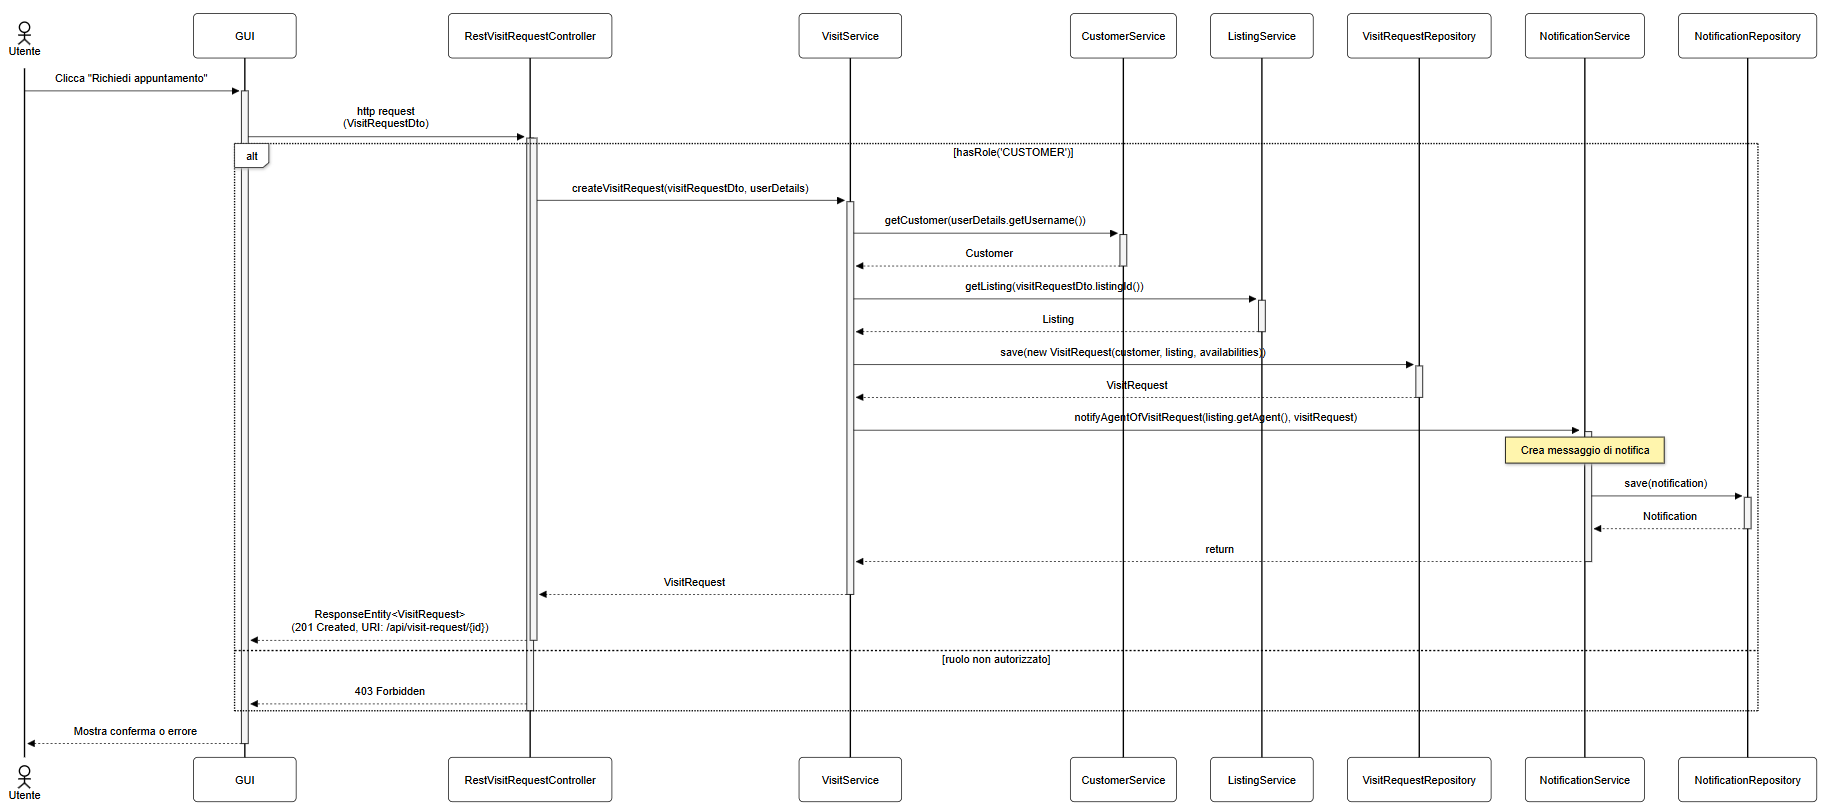
\includegraphics[width=\textwidth]{assets/diagrams/sequence/fissa-appuntamento.png}
    }
        \caption{Diagramma di sequenza del caso d'uso Fissa Appuntamento.}
    \label{fig:Diagramma di sequenza del caso d'uso Fissa Appuntamento}
\end{figure}

\begin{figure}[H]
    \adjustbox{width=1.4\textwidth,center}{
        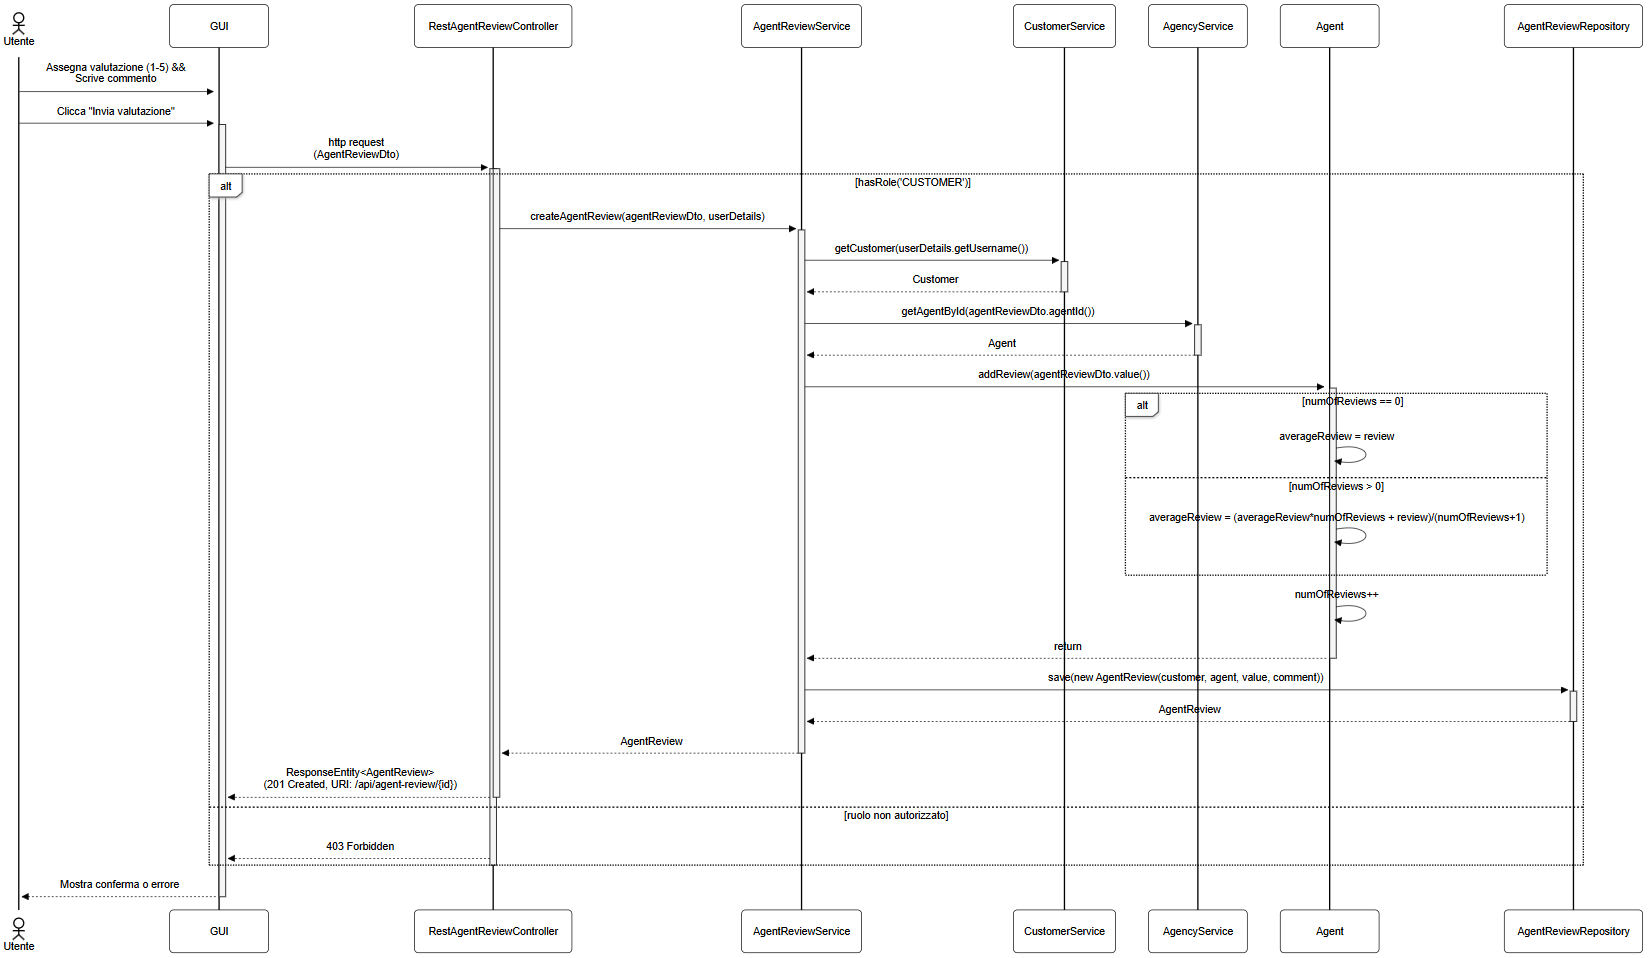
\includegraphics[width=\textwidth]{assets/diagrams/sequence/valuta-agente.png}
    }
        \caption{Diagramma di sequenza del caso d'uso Valuta Agente.}
    \label{fig:Diagramma di sequenza del caso d'uso Valuta Agente}
\end{figure}

\begin{figure}[H]
    \adjustbox{width=1.4\textwidth,center}{
        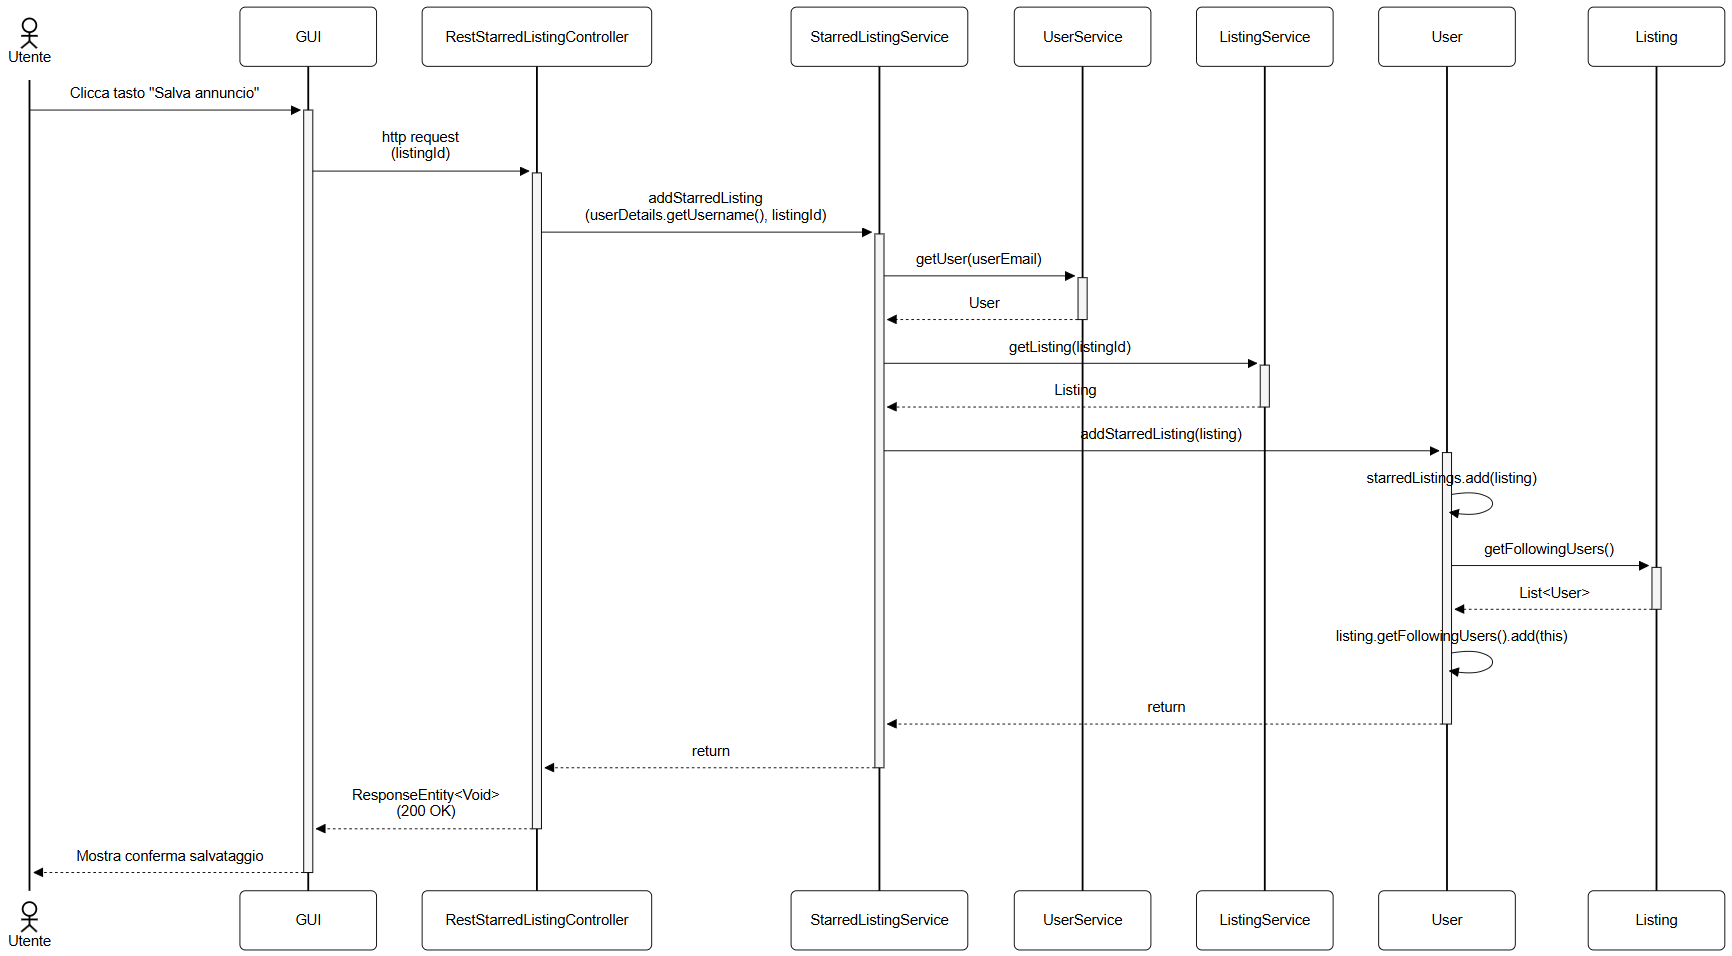
\includegraphics[width=\textwidth]{assets/diagrams/sequence/salva-annuncio.png}
    }
    \caption{Diagramma di sequenza del caso d'uso Salva Annuncio.}
    \label{fig:Diagramma di sequenza del caso d'uso Salva Annuncio}
\end{figure}

\section{Design del front-end}

\chapter{Testing del sistema}
L'attività di testing rappresenta una fase cruciale nel ciclo 
di sviluppo del software, in quanto garantisce la qualità, 
l'affidabilità e la robustezza del sistema. Questo capitolo 
illustra l'approccio metodologico e gli strumenti utilizzati per 
la verifica del corretto funzionamento del sistema.

Il testing é stato organizzato su due livelli: test unitari per
testare in isolamento la business logic; test di API tramite collection
di Postman. Tuttavia, il test di API é ancora in fase di sviluppo ed
é pertanto incompleto. Le collection sono, ad oggi, uno strumento per
gli sviluppatori per provare il funzionamento degli endpoint in modo rapido.
É previsto di rendere le collection degli effettivi test di API.

\section{Testing unitario}
Il concetto di unitá é da sempre flessibile: le unitá vanno definite
in base al contesto. Nel contesto di un sistema come DietiEstates25, é
una scelta comune quella di considerare i Service e le funzioni ausiliare
le unitá di testing.
Il testing dei Service permette di testare il funzionamento della business
logic. É anche importante specificare che, nel testing di un software sviluppato
su un framework come Spring Boot, testare meccanismi forniti da Spring Boot o
moduli terzi é chiaramente inutile.
Il testing delle funzioni ausiliare permette di assicurarsi che tali funzioni,
spesso largamente utilizzate nel codice, siano corrette. La correttezza di tali funzioni
permette di risparmiare potenzialmente tanto tempo in fase di debugging.

Si è deciso di usare una libreria di faking (Faker) per aumentare la casualitá dei campioni.

A valle di queste considerazioni, descriviamo il testing effettuato.
I test sono stati creati attraverso la piattaforma JUnit5.
\subsection{JwtUtil.isTokenValid}
Questo metodo della classe di gestione di JWT é di cruciale importanza per quanto
riguarda l'intero sistema di autorizzazione del backend.

\begin{table}[h!]
    \centering
    \renewcommand{\arraystretch}{1.4}
    \begin{tabularx}{\textwidth}{|X|X|X|}
    \hline
    \textbf{Parametro} & \textbf{Classe di Equivalenza} & \textbf{Validità} \\
    \hline
    \texttt{token} & Stringa vuota & Non valida \\
    \hline
    \texttt{token} & Token valido & Valida \\
    \hline
    \texttt{token} & Token non valido & Non valida \\
    \hline
    \texttt{token} & Token scaduto & Non valida \\
    \hline
    \texttt{UserDetails} & UserDetails valido & Valida \\
    \hline
    \end{tabularx}
    \caption{Classi di equivalenza per il testing black-box dei parametri \texttt{token} e \texttt{UserDetails}}
\end{table}

Note: 
\begin{list}{$\cdot$}{}
    \item Poiché isTokenValid viene chiamata una volta che si è 
    verificato che token è diverso da null in JwtAuthFilter, si 
    è deciso di evitare il testing sulla classe di equivalenza 
    null.
    \item Poiché isTokenValid viene chiamata una volta che si è 
    verificato che UserDetails è diverso da null (dal metodo 
    loadUserByUsername(username) di UserDetails invocato in 
    JwtAuthFilter), si è deciso di evitare il testing sulla 
    classe di equivalenza null.
    \item Si è deciso di creare una classe copia per il testing 
    a causa della non iniettabilità, per motivi di sicurezza, 
    della classe di produzione.
\end{list}

\noindent
I casi di test, secondo strategia R-WECT, sono:
\begin{table}[h!]
    \centering
    \renewcommand{\arraystretch}{1.4}
    \begin{tabularx}{\textwidth}{|X|X|X|}
    \hline
    \textbf{Token} & \textbf{UserDetails} & \textbf{Risultato Atteso} \\
    \hline
    Stringa vuota & UserDetails valido & \texttt{InvalidTokenException} \\
    \hline
    Token valido & UserDetails valido & \texttt{true} \\
    \hline
    Token scaduto & UserDetails valido & \texttt{InvalidTokenException} \\
    \hline
    Token non valido & UserDetails valido & \texttt{InvalidTokenException} \\
    \hline
    \end{tabularx}
    \caption{Casi di test secondo la strategia R-WECT}
\end{table}

\newpage
\lstinputlisting[
    style=javaStyle, 
    caption={La classe di testing per JwtUtil.isTokenValid}, 
]{assets/code/jwt-test.java}
    
\subsection{AgentReviewService::createAgentReview}
AgentReviewService::createAgentReview(AgentReviewDto, UserDetails) é invocato in contesti in 
cui UserDetails é sempre ben definito, ovvero sempre diverso da null e sempre contenente 
informazioni di utente esistente.
AgentReview Dto è costituito da:
\begin{list}{$\cdot$}{}
    \item agentId: é garantito dal validator (Hibernate Validator) che non sia null o empty-string
    \item value: é garantito dal validator che non sia null e che sia compreso tra 1 e 5
    \item comment
\end{list}

È stato scelto, per la definizione dei casi di test, un approccio functionality-based, 
in modo da considerare solo i casi di test reali. I casi di test sono:
\begin{table}[h!]
    \centering
    \renewcommand{\arraystretch}{1.4}
    \begin{tabularx}{\textwidth}{|X|X|}
    \hline
    \textbf{Agent ID} & \textbf{Risultato Atteso} \\
    \hline
    Agent ID errato & \texttt{EntityNotExistsException} \\
    \hline
    Agent ID corretto & \texttt{AgentReview} \\
    \hline
    \end{tabularx}
    \caption{Casi di test per Agent ID}
\end{table}

\newpage
\lstinputlisting[
    style=javaStyle, 
    caption={La classe di testing per AgentReviewService::createAgentReview}, 
]{assets/code/agent-review-test.java}
    
\subsection{StarredListingService::addStarredListing}
StarredListingService::addStarredListing(String userEmail, String listingId) é invocato 
in contesti in cui la validitá di userEmail é garantita. Per quanto riguarda 
listingId, il validator garantisce che, al momento della chiamata di 
questo metodo, listingId sia non nulla e non vuota.

A questo punto, le classi di equivalenza da considerare per listingId sono:
\begin{table}[h!]
    \centering
    \renewcommand{\arraystretch}{1.4}
    \begin{tabularx}{\textwidth}{|X|X|}
    \hline
    \textbf{listingId} & \textbf{Validità} \\
    \hline
    listingId errato & Non valida \\
    \hline
    listingId valido & Valida \\
    \hline
    \end{tabularx}
    \caption{Classi di equivalenza per \texttt{listingId}}
\end{table}
    
I casi di test sono:
\begin{table}[h!]
    \centering
    \renewcommand{\arraystretch}{1.4}
    \begin{tabularx}{\textwidth}{|X|X|}
    \hline
    \textbf{listingId} & \textbf{Risultato Atteso} \\
    \hline
    listingId errato & \texttt{EntityNotExistsException} \\
    \hline
    listingId valido & \texttt{void}, e il listing compare tra gli \texttt{starredListings} dell’utente \\
    \hline
    \end{tabularx}
    \caption{Casi di test per \texttt{listingId}}
\end{table}

\newpage
\lstinputlisting[
    style=javaStyle, 
    caption={La classe di testing per StarredListingService::addStarredListing}, 
]{assets/code/starred-listings-test.java}
    
\subsection{VisitService::createVisitRequest}
VisitService::createVisitRequest(VisitRequestDto visitRequestDto, UserDetails userDetails) 
é invocata in contesti in cui la validitá di userDetails é garantita. 
Per quanto riguarda visitRequestDto(String listingId, List$<$Availability$>$ availabilities), 
é garantito che:
\begin{list}{$\cdot$}{}
    \item listingId sia non nullo e non vuoto.
    \item availabilities sia non nullo e che le sue TimeSlot siano 
    valide (ció é garantito da Jackson).
\end{list}

Le classi di equivalenza sono quindi:
\begin{table}[H]
    \centering
    \renewcommand{\arraystretch}{1.4}
    \begin{tabularx}{\textwidth}{|X|X|X|}
    \hline
    \textbf{Parametro} & \textbf{Classe di Equivalenza} & \textbf{Validità} \\
    \hline
    \texttt{listingId} & listingId errato & Non valida \\
    \hline
    \texttt{listingId} & listingId valido & Valida \\
    \hline
    \texttt{availabilities} & Lista vuota & Valida \\
    \hline
    \texttt{availabilities} & Timeslot validi & Valida \\
    \hline
    \end{tabularx}
    \caption{Classi di equivalenza per \texttt{listingId} e \texttt{availabilities}}
\end{table}

I casi di test, secondo strategia R-WECT, sono:
\begin{table}[H]
    \centering
    \renewcommand{\arraystretch}{1.4}
    \begin{tabularx}{\textwidth}{|X|X|X|}
    \hline
    \textbf{listingId} & \textbf{availabilities} & \textbf{Risultato Atteso} \\
    \hline
    listingId errato & Timeslot validi & \makecell[l]{\texttt{EntityNotExists}\\\texttt{Exception}} \\
    \hline
    listingId valido & Lista vuota & \texttt{VisitRequest} senza disponibilità specificate \\
    \hline
    listingId valido & Timeslot validi & \texttt{VisitRequest} con le disponibilità specificate \\
    \hline
    \end{tabularx}
    \caption{Casi di test secondo la strategia R-WECT per \texttt{listingId} e \texttt{availabilities}}
    \end{table}

\newpage
\lstinputlisting[
    style=javaStyle, 
    caption={La classe di testing per VisitService::createVisitRequest}, 
]{assets/code/visit-request-test.java}

\end{document}
